\addtocontents{xms}{\protect\addvspace{10pt}}
\chapter{Exemples Resolts amb Python}\label{chap:python-exemples}


\section{Exemples del capítol \ref*{ch:fonaments}}

\hypertarget{exemple:MillmanBateries}{\subsection{Exemple \ref*{ex:MillmanBateries} \MillmanBateries}}

En el llistat \vref{lst:MillmanBateries} es pot veure el programa utilitzat per resoldre l'exemple \vref{ex:MillmanBateries}. La resolució es fa de dues maneres: fent ús primer de les funcions \texttt{z\_parallel} i \texttt{millman} del mòdul \texttt{qed.eng\_elec}, i fent servir després les classes \texttt{Network}, \texttt{VoltageSource} i \texttt{Impedance}  del mateix mòdul.
\lstset{
	language=Python,
	numbers=left,
	frame=lines,
	morekeywords=[1]{as,None,match,case,with}
}
\lstinputlisting[caption={Python --- Exemple \ref*{ex:MillmanBateries} \MillmanBateries},label=lst:MillmanBateries]{Python/exemples_resolts/Exemple-1-1.py}

Quan s'executa aquest programa, el resultat que s'obté és:
\lstset{
	language=,
	numbers=none,
	frame=none
}
\begin{lstlisting}
Teorema de Millman
------------------
Z_Th = 11.3270 mΩ
E_Th = 125.0562 V
Y_No = 88.28 S
J_No = 11.04 kA
I = 2.5006 A
U = 125.03 V

Mètode dels nusos
------------------
Z_Th = 11.3270 mΩ
E_Th = 125.0562 V
Y_No = 88.28 S
J_No = 11.04 kA
I = 2.5006 A
U = 125.03 V
\end{lstlisting} 


\hypertarget{exemple:MillmanTrifNeutre}{\subsection{Exemple \ref*{ex:MillmanTrifNeutre} \MillmanTrifNeutre}}

En el llistat \vref{lst:MillmanTrifNeutre} es pot veure el programa utilitzat per resoldre l'exemple \vref{ex:MillmanTrifNeutre}. La resolució es fa de dues maneres: usant primer la funció \texttt{millman} del mòdul \texttt{qed.eng\_elec}, i fent servir després les classes \texttt{Network},  \texttt{VoltageSource} i \texttt{Impedance}  del mateix mòdul. Es fa servir també la classe \texttt{Complex} del mòdul \texttt{qed.utils}.
\lstset{
	language=Python,
	numbers=left,
	frame=lines,
	morekeywords=[1]{as,None,match,case,with}
}
\lstinputlisting[caption={Python --- Exemple \ref*{ex:MillmanTrifNeutre} \MillmanTrifNeutre},label=lst:MillmanTrifNeutre]{Python/exemples_resolts/Exemple-1-2.py}

Quan s'executa aquest programa, el resultat que s'obté és:
\lstset{
	language=,
	numbers=none,
	frame=none
}
\begin{lstlisting}
Teorema de Millman
------------------------------
U_GN = 33.3433∠13.17° V
I_A  = 3953.6056∠-2.20° A
I_B  = 3174.7573∠-125.49° A
I_C  = 3453.8265∠127.59° A
I_N  = 0.7249∠13.17° A

Mètode dels nusos
------------------------------
U_GN = 33.3433∠13.17° V
I_A  = 3953.6056∠-2.20° A
I_B  = 3174.7573∠-125.49° A
I_C  = 3453.8265∠127.59° A
I_N  = 0.7249∠13.17° A
\end{lstlisting} 


\hypertarget{exemple:Superposicio}{\subsection{Exemple \ref*{ex:Superposicio} \Superposicio}}

En el llistat \vref{lst:Superposicio} es pot veure el programa utilitzat per resoldre l'exemple \vref{ex:Superposicio}. La resolució es fa amb les classes \texttt{Network}, \texttt{VoltageSource}, \texttt{CurrentSource} i \texttt{Impedance} del mòdul \texttt{qed.eng\_elec}, obtenint el corrent buscat de forma directa, sense necessitat d'utilitzar el teorema de la superposició. Es fa servir també la classe \texttt{Complex} del mòdul \texttt{qed.utils}.
\lstset{
	language=Python,
	numbers=left,
	frame=lines,
	morekeywords=[1]{as,None,match,case,with}
}
\lstinputlisting[caption={Python --- Exemple \ref*{ex:Superposicio} \Superposicio},label=lst:Superposicio]{Python/exemples_resolts/Exemple-1-4.py}

Quan s'executa aquest programa, el resultat que s'obté és:
\lstset{
	language=,
	numbers=none,
	frame=none
}
\begin{lstlisting}
Corrent pel condensador: 2.907∠26.57° A
\end{lstlisting} 


\hypertarget{exemple:CarDescRL}{\subsection{Exemple \ref*{ex:CarDescRL} \CarDescRL}}

En el llistat \vref{lst:CarDescRL} es pot veure el programa utilitzat per resoldre l'exemple \vref{ex:CarDescRL}. La resolució es fa utilitzant funcions del mòdul numèric \texttt{numpy} i del mòdul gràfic  \texttt{matplotlib}.
\lstset{
	language=Python,
	numbers=left,
	frame=lines,
	morekeywords=[1]{as,None,match,case,with}
}
\lstinputlisting[caption={Python --- Exemple \ref*{ex:CarDescRL} \CarDescRL},label=lst:CarDescRL]{Python/exemples_resolts/Exemple-1-8.py}

Quan s'executa aquest programa, el resultat que s'obté és:
\lstset{
	language=,
	numbers=none,
	frame=none
}
\begin{lstlisting}[mathescape=true]
$ 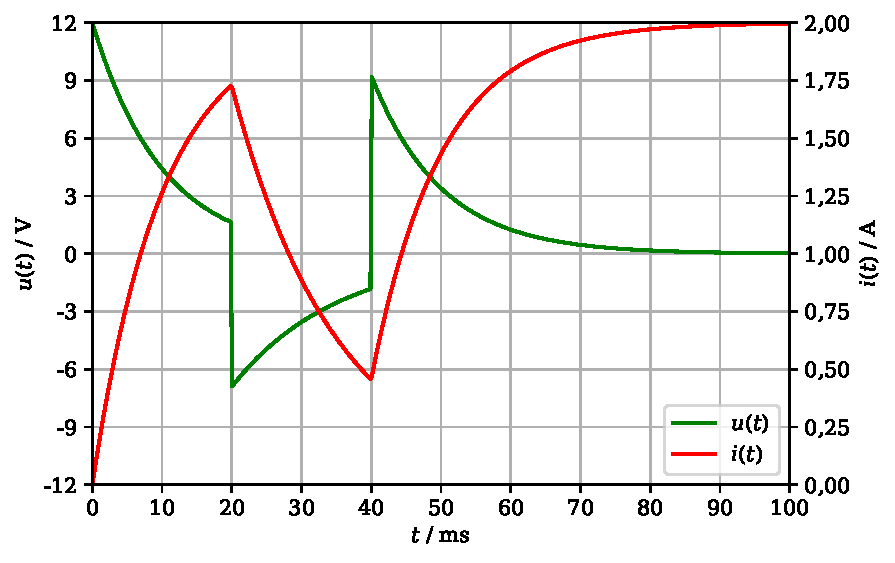
\includegraphics{Cap-PythonExemp-CarDescRL.pdf} $
\end{lstlisting}


\hypertarget{exemple:CurtcircuitRL}{\subsection{Exemple \ref*{ex:CurtcircuitRL} \CurtcircuitRL}}
En el llistat \vref{lst:CurtcircuitRL} es pot veure el programa utilitzat per resoldre l'exemple \vref{ex:CurtcircuitRL}. La resolució es fa utilitzant funcions del mòdul numèric \texttt{numpy} i del mòdul gràfic  \texttt{matplotlib}.
\lstset{
	language=Python,
	numbers=left,
	frame=lines,
	morekeywords=[1]{as,None,match,case,with}
}

\pagebreak

\lstinputlisting[caption={Python --- Exemple \ref*{ex:CurtcircuitRL} \CurtcircuitRL},label=lst:CurtcircuitRL]{Python/exemples_resolts/Exemple-1-9.py}

Quan s'executa aquest programa, el resultat que s'obté és:
\lstset{
	language=,
	numbers=none,
	frame=none
}

\begin{lstlisting}[mathescape=true]
	
Intensitat simètrica eficaç = 25423.0955 A

Intensitat asimètrica de pic = 71.9 kA

Intensitat asimètrica eficaç = 44.0 kA




$ 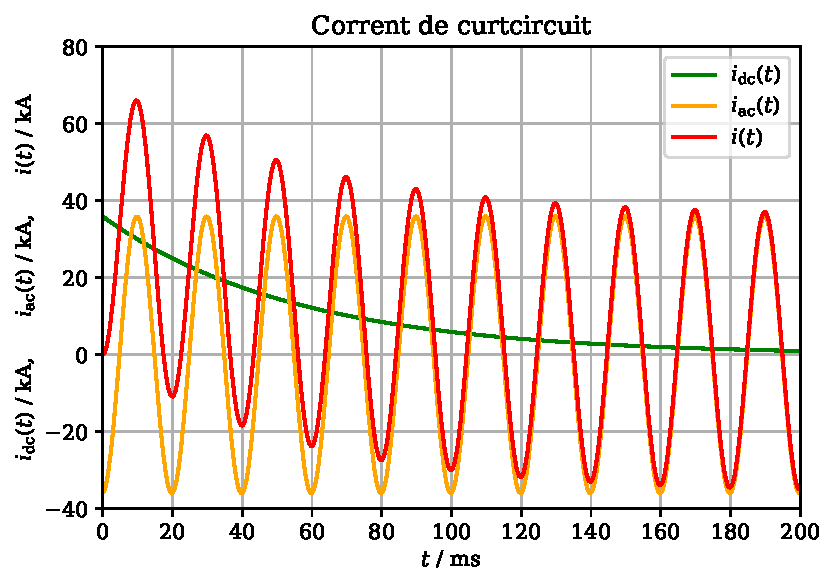
\includegraphics{Cap-PythonExemp-CurtcircuitRL.pdf} $
\end{lstlisting}


\hypertarget{exemple:CurtcircuitPicRL}{\subsection{Exemple \ref*{ex:CurtcircuitPicRL} \CurtcircuitPicRL}}
En el llistat \vref{lst:CurtcircuitPicRL} es pot veure el programa utilitzat per resoldre l'exemple \vref{ex:CurtcircuitPicRL}. La resolució es fa fent ús de funcions del mòdul numèric \texttt{numpy}, i la funció \texttt{minimize\_scalar} del mòdul  \texttt{scipy.optimize}, la qual troba mínims locals d'una funció; com que en aquest cas  el que es vol trobar és un màxim local, cal posar un signe negatiu davant de la funció que es passa a \texttt{minimize\_scalar} i un signe negatiu davant de la solució obtinguda.
\lstset{
	language=Python,
	numbers=left,
	frame=lines,
	morekeywords=[1]{as,None,match,case,with}
}
\lstinputlisting[caption={Python --- Exemple \ref*{ex:CurtcircuitPicRL} \CurtcircuitPicRL},label=lst:CurtcircuitPicRL]{Python/exemples_resolts/Exemple-1-10.py}

Quan s'executa aquest programa, el resultat que s'obté és:
\lstset{
	language=,
	numbers=none,
	frame=none
}
\begin{lstlisting}
Factor κ (CEI 60909-1) = 1.8452
Intensitat asimètrica de pic (CEI 60909-1) = 66.3 kA
Intensitat asimètrica de pic (exacta) = 66075.5 A (t = 9.6650 ms)
\end{lstlisting}


\hypertarget{exemple:Malles}{\subsection{Exemple \ref*{ex:Malles} \Malles}}
En el llistat \vref{lst:Malles} es pot veure el programa utilitzat per resoldre l'exemple \vref{ex:Malles}. La resolució es fa de dues maneres: fent ús  primer de la funció \texttt{solve} del mòdul \texttt{scipy.linalg}, i fent servir després les classes \texttt{Network}, \texttt{VoltageSource} i \texttt{Impedance} del mòdul \texttt{qed.eng\_elc}.
\lstset{
	language=Python,
	numbers=left,
	frame=lines,
	morekeywords=[1]{as,None,match,case,with}
}
\lstinputlisting[caption={Python --- Exemple \ref*{ex:Malles} \Malles},label=lst:Malles]{Python/exemples_resolts/Exemple-1-11.py}

Quan s'executa aquest programa, el resultat que s'obté és:
\lstset{
	language=,
	numbers=none,
	frame=none
}
\begin{lstlisting}
Resolució algebraica
--------------------
I1 = 2.75 A
I2 = -0.50 A
I3 = 2.25 A
I4 = 0.50 A
I5 = 1.25 A
I6 = 0.75 A

Mètode dels nusos
-----------------
I1 = 2.75 A
I2 = -0.50 A
I3 = 2.25 A
I4 = 0.50 A
I5 = 1.25 A
I6 = 0.75 A
\end{lstlisting} 



\section{Exemples del capítol \ref*{sec:ch-calc-bas}}

\hypertarget{exemple:TriangleEstrella}{\subsection{Exemple \ref*{ex:TriangleEstrella} \TriangleEstrella}}
En el llistat \vref{lst:TriangleEstrella} es pot veure el programa utilitzat per resoldre l'exemple \vref{ex:TriangleEstrella}. Es fa servir la funció \texttt{D\_to\_Y} del mòdul \texttt{qed.eng\_elec} per fer la transformació de triangle a estrella.
\lstset{
	language=Python,
	numbers=left,
	frame=lines,
	morekeywords=[1]{as,None,match,case,with}
}
\lstinputlisting[caption={Python --- Exemple \ref*{ex:TriangleEstrella} \TriangleEstrella},label=lst:TriangleEstrella]{Python/exemples_resolts/Exemple-2-2.py}

Quan s'executa aquest programa, el resultat que s'obté és:
\lstset{
	language=,
	numbers=none,
	frame=none
}
\begin{lstlisting}
Z_A = (4-2j) Ω
Z_B = (4-2j) Ω
Z_C = (-2-4j) Ω
\end{lstlisting}


\hypertarget{exemple:ResCircPotAbs}{\subsection{Exemple \ref*{ex:ResCircPotAbs} \ResCircPotAbs}}
En el llistat \vref{lst:ResCircPotAbs} es pot veure el programa utilitzat per resoldre l'exemple \vref{ex:ResCircPotAbs}. Es fa servir la funció \texttt{ezs\_u} del mòdul \texttt{qed.eng\_elec} per calcular la tensió de la càrrega.
\lstset{
	language=Python,
	numbers=left,
	frame=lines,
	morekeywords=[1]{as,None,match,case,with}
}
\lstinputlisting[caption={Python --- Exemple \ref*{ex:ResCircPotAbs} \ResCircPotAbs},label=lst:ResCircPotAbs]{Python/exemples_resolts/Exemple-2-3.py}

Quan s'executa aquest programa, el resultat que s'obté és:
\lstset{
	language=,
	numbers=none,
	frame=none
}
\begin{lstlisting}
U   = 0.3165+0.0874j
I   = 2.1259-0.8346j
Z_S = 0.1150+0.0863j
\end{lstlisting}

Es pot observar que algun dels valors obtinguts no és exactament igual al valor obtingut en la resolució manual; la diferència es deu al fet que en la resolució manual s'han utilitzat només quatre xifres decimals, mentre que el programa treballa sempre amb tota la precisió de les variables (típicament, setze xifres decimals).



\section{Exemples del capítol \ref*{sec:ch-comp-sim}}

\hypertarget{exemple:ImpedEquil}{\subsection{Exemple \ref*{ex:ImpedEquil} \ImpedEquil}}
En el llistat \vref{lst:ImpedEquil} es pot veure el programa utilitzat per resoldre l'exemple \vref{ex:ImpedEquil}. S'usen funcions relatives a les components simètriques del mòdul \texttt{qed.eng\_elec} per fer els càlculs. Es fa servir també la classe \texttt{Complex} del mòdul \texttt{qed.utils}.
\lstset{
	language=Python,
	numbers=left,
	frame=lines,
	morekeywords=[1]{as,None,match,case,with}
}
\lstinputlisting[caption={Python --- Exemple \ref*{ex:ImpedEquil} \ImpedEquil},label=lst:ImpedEquil]{Python/exemples_resolts/Exemple-3-1.py}

Quan s'executa aquest programa, el resultat que s'obté és:
\lstset{
	language=,
	numbers=none,
	frame=none
}
\begin{lstlisting}
U_AB = 2760.00∠0.00° V
U_BC = 1840.00∠-124.23° V
U_CA = 2300.00∠138.59° V

U_AB_1 = 2267.09∠5.04° V
U_AB_2 = 539.77∠-21.66° V
U_AB_0 = 0.00∠153.43° V

U_AG_1 = 1308.91∠-24.96° V
U_AG_2 = 311.64∠8.34° V
U_AG_0 = 0.00∠0.00° V

I_A_1 = 130.89∠-24.96° A
I_A_2 = 31.16∠8.34° A
I_A_0 = 0.00∠0.00° A

S_3F = 543.11+0.00j kVA

U_AG = 1578.66∠-18.74° V
U_BG = 1362.86∠-158.16° V
U_CG = 1039.96∠102.78° V

U_AG = 1578.66∠-18.74° V
U_BG = 1362.86∠-158.16° V
U_CG = 1039.96∠102.78° V
\end{lstlisting}


\hypertarget{exemple:ImpedDesequil}{\subsection{Exemple \ref*{ex:ImpedDesequil} \ImpedDesequil}}
En el llistat \vref{lst:ImpedDesequil} es pot veure el programa utilitzat per resoldre l'exemple \vref{ex:ImpedDesequil}. S'usen funcions relatives a les components simètriques del mòdul \texttt{qed.eng\_elec} per fer els càlculs. Es fa servir també la classe \texttt{Complex} del mòdul \texttt{qed.utils}.
\lstset{
	language=Python,
	numbers=left,
	frame=lines,
	morekeywords=[1]{as,None,match,case,with}
}
\lstinputlisting[caption={Python --- Exemple \ref*{ex:ImpedDesequil} \ImpedDesequil},label=lst:ImpedDesequil]{Python/exemples_resolts/Exemple-3-2.py}

Quan s'executa aquest programa, el resultat que s'obté és:
\lstset{
	language=,
	numbers=none,
	frame=none
}
\begin{lstlisting}
U_AB = 2760.00∠0.00° V
U_BC = 1840.00∠-124.23° V
U_CA = 2300.00∠138.59° V

U_AN = 1101.65∠-14.54° V
U_BN = 1716.07∠-170.72° V
U_CN = 1408.22∠117.89° V

U_AN_1 = 1308.91∠-24.96° V
U_AN_2 = 311.64∠8.34° V
U_AN_0 = 486.68∠151.73° V

U_GN = 486.68∠151.73° V
\end{lstlisting}




\section{Exemples del capítol \ref*{sec:ch-series-fourier}}

\hypertarget{exemple:CircuitFourier}{\subsection{Exemple \ref*{ex:CircuitFourier} \CircuitFourier}}
En el llistat \vref{lst:CircuitFourier} es pot veure el programa utilitzat per resoldre l'exemple \vref{ex:CircuitFourier}. La resolució es fa usant funcions del mòdul numèric \texttt{numpy} i del mòdul gràfic  \texttt{matplotlib}.
\lstset{
	language=Python,
	numbers=left,
	frame=lines,
	morekeywords=[1]{as,None,match,case,with}
}
\lstinputlisting[caption={Python --- Exemple \ref*{ex:CircuitFourier} \CircuitFourier},label=lst:CircuitFourier]{Python/exemples_resolts/Exemple-4-3.py}

Quan s'executa aquest programa, el resultat que s'obté és:
\lstset{
	language=,
	numbers=none,
	frame=none
}
\begin{lstlisting}[mathescape=true]
I = 0.5505 A
P = 3.03 W
P = 3.03 W


$ 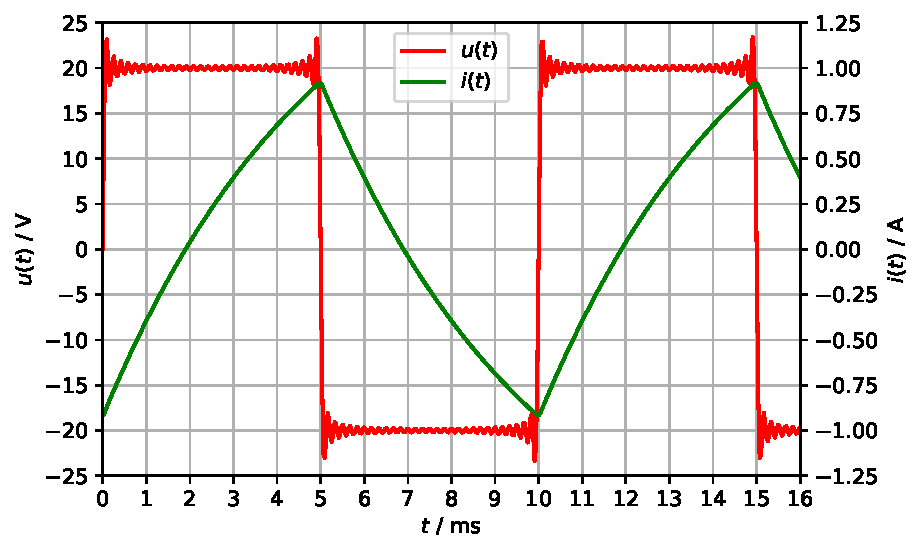
\includegraphics{Cap-PythonExemp-CircuitFourier-1.pdf} $


$ 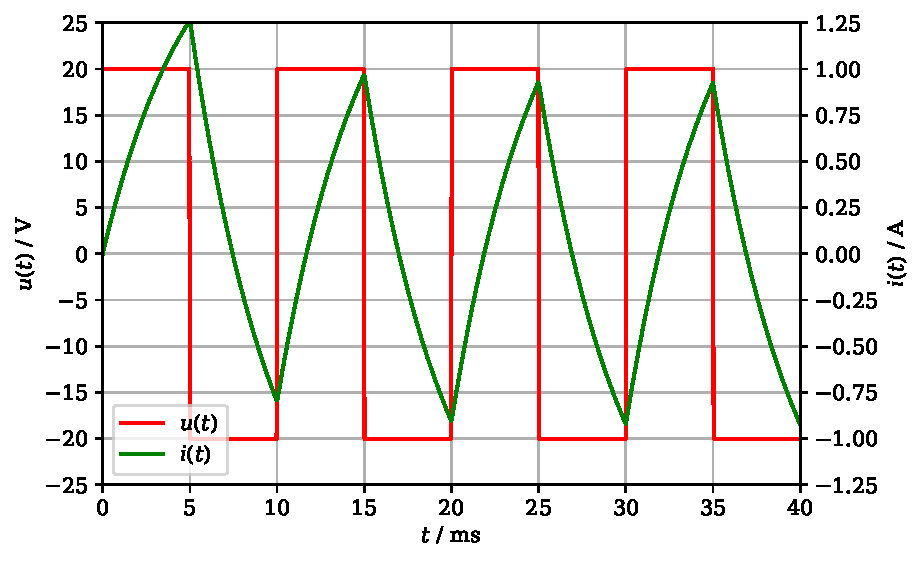
\includegraphics{Cap-PythonExemp-CircuitFourier-2.pdf} $


$ 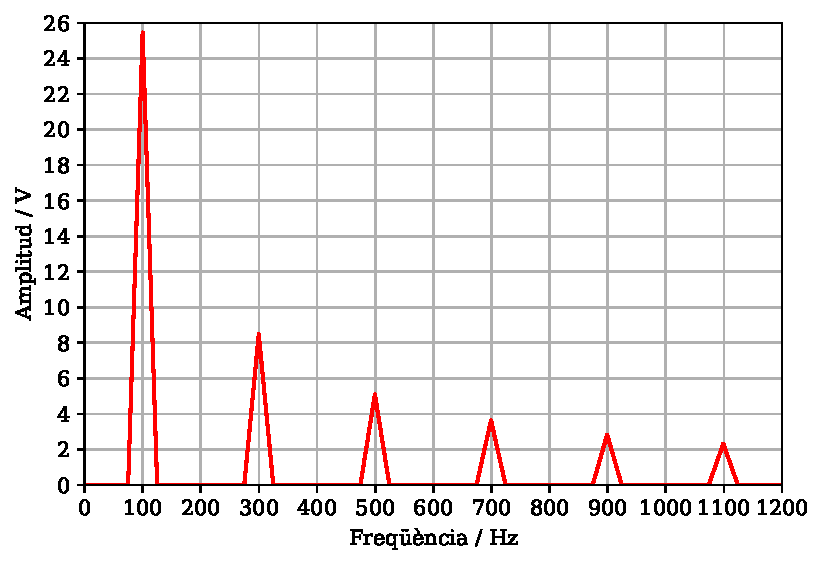
\includegraphics{Cap-PythonExemp-CircuitFourier-3.pdf} $
\end{lstlisting} 

L'última gràfica és una ampliació respecte de l'exemple resolt a mà. S'utilitzen les funcions \texttt{fft.rfft} i \texttt{fft.rfftfreq} del mòdul numèric \texttt{numpy} per aplicar la transformada ràpida de Fourier a l'ona rectangular de tensió. El que s'obté correspon a la sèrie de Fourier d'aquesta ona calculada en l'exemple resolt a  mà, és a dir, els termes de freqüència \qty{100}{Hz}, \qty{300}{Hz}, \qty{500}{Hz}, etc., d'una amplitud respectiva de \qty{25,4648}{V}, \qty{8,4883}{V}, \qty{5,0292}{V}, etc. L'ús d'aquestes dues funcions no és senzill, i cal llegir amb atenció la documentació del mòdul \texttt{numpy}; en particular, cal tenir en compte que per obtenir valors correctes és necessari utilitzar un temps total que sigui un múltiple enter del període de l'ona (\qty{40}{ms} en aquest cas).


\section{Exemples del capítol \ref*{sec:ch-laplace}}

\hypertarget{exemple:CircuitLaplace}{\subsection{Exemple \ref*{ex:CircuitLaplace} \CircuitLaplace}}
En el llistat \vref{lst:CircuitLaplace} es pot veure el programa utilitzat per resoldre l'exemple \vref{ex:CircuitLaplace}. La resolució es fa fent ús de funcions del mòdul de matemàtica simbòlica \texttt{sympy}, del mòdul numèric \texttt{numpy} i del mòdul gràfic  \texttt{matplotlib}. 

Del mòdul \texttt{sympy} es fa servir bàsicament la funció \texttt{Eq} per definir equacions,  la funció \texttt{solve} per aïllar una variable d'una equació, la funció \texttt{subs} per substituir  una variable per la seva expressió en una equació, i la   funció \texttt{inverse\_laplace\_transform} per obtenir la transformada inversa de Laplace. 

Aquesta  darrera funció requereix que els valors numèrics implicats siguin exactes, i és per això que cal fer servir la funció \texttt{Rational} quan tenim valors no enters; per exemple, en lloc de \texttt{L = 250e-3} cal utilitzar \texttt{sympy.Rational(250, 1000)}, i el lloc de \texttt{iL\_0 =  U\_bat/(R\_bat + R\_3)} cal usar \texttt{iL\_0 = sympy.Rational(U\_bat, R\_bat + R\_3)}.
\pagebreak

\lstset{
	language=Python,
	numbers=left,
	frame=lines,
	morekeywords=[1]{as,None,match,case,with}
}
\lstinputlisting[caption={Python --- Exemple \ref*{ex:CircuitLaplace} \CircuitLaplace},label=lst:CircuitLaplace]{Python/exemples_resolts/Exemple-5-3.py}

Quan s'executa aquest programa, el resultat que s'obté és:
\lstset{
	language=,
	numbers=none,
	frame=none
}
\begin{lstlisting}[mathescape=true]
iL_0 = 4 A
uC_0 = 100 V
iL(s) = 4*(s + 1075)/(s**2 + 1475*s + 700000)
iL(t) = 4*(3*sqrt(111)*sin(75*sqrt(111)*t/2) + 37*cos(75*sqrt(111)*t/2))*exp(-1475*t/2)/37
iL(0) = 4 A

$ 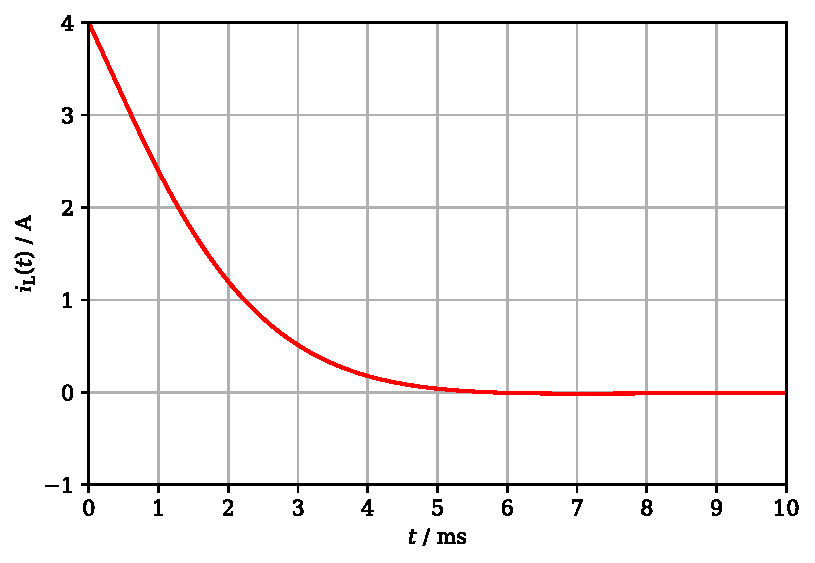
\includegraphics{Cap-PythonExemp-CircuitLaplace.pdf} $
\end{lstlisting} 



\hypertarget{exemple:CircuitLaplaceNul}{\subsection{Exemple \ref*{ex:CircuitLaplaceNul} \CircuitLaplaceNul}}

En el llistat \vref{lst:CircuitLaplaceNul} es pot veure el programa utilitzat per resoldre l'exemple \vref{ex:CircuitLaplaceNul}. La resolució es fa emprant funcions del mòdul de matemàtica simbòlica \texttt{sympy}, del mòdul numèric \texttt{numpy} i del mòdul gràfic  \texttt{matplotlib}. 

Tal com s'ha dit en l'exemple anterior, la funció \texttt{inverse\_laplace\_transform} del mòdul \texttt{sympy}  requereix que els valors numèrics implicats siguin exactes, i és per això que cal fer servir \texttt{sympy.sqrt(2)} i \texttt{sympy.pi} per representar respectivament  $\sqrt{2}$ i $\piup$.

\lstset{
	language=Python,
	numbers=left,
	frame=lines,
	morekeywords=[1]{as,None,match,case,with}
}
\lstinputlisting[caption={Python --- Exemple \ref*{ex:CircuitLaplaceNul} \CircuitLaplaceNul},label=lst:CircuitLaplaceNul]{Python/exemples_resolts/Exemple-5-4.py}


Quan s'executa aquest programa, el resultat que s'obté és:
\lstset{
	language=,
	numbers=none,
	frame=none
}
\begin{lstlisting}[mathescape=true]
uC(t) = 11000*sqrt(2)*((10*pi*sin(100*pi*t) + (50 - pi**2)*cos(100*pi*t))*exp(500*t) - (pi**2 + 50)*sin(500*t) + (-50 + pi**2)*cos(500*t))*exp(-500*t)/(pi**4 + 2500)

$ 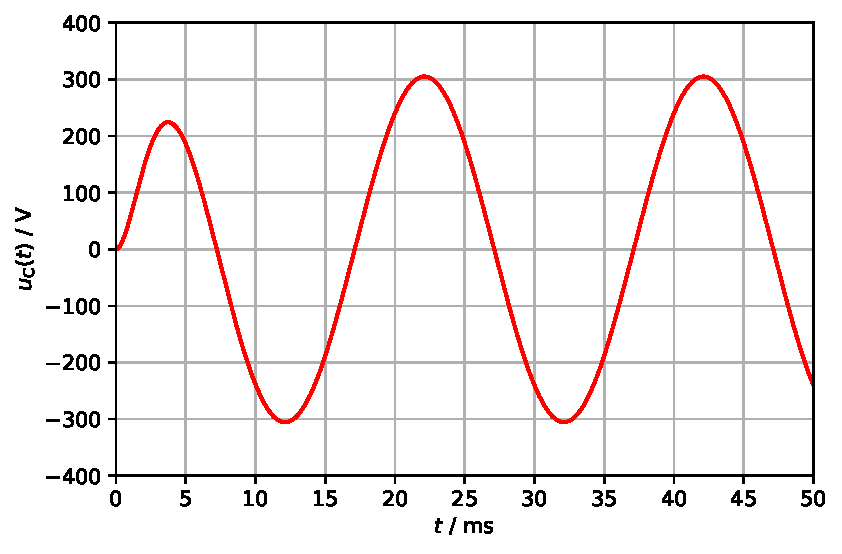
\includegraphics{Cap-PythonExemp-CircuitLaplaceNul.pdf} $
\end{lstlisting} 



\section{Exemples del capítol \ref*{sec:ch-cables}}

\hypertarget{exemple:CaigudaDeTensio}{\subsection{Exemple \ref*{ex:CaigudaDeTensio} \CaigudaDeTensio}}
En el llistat \vref{lst:CaigudaDeTensio} es pot veure el programa utilitzat per resoldre l'exemple \vref{ex:CaigudaDeTensio}. La resolució es fa usant la funció \texttt{voltage\_drop} i la constant \texttt{SQRT3} del mòdul \texttt{qed.eng\_elec}.
\lstset{
	language=Python,
	numbers=left,
	frame=lines,
	morekeywords=[1]{as,None,match,case,with}
}
\lstinputlisting[caption={Python --- Exemple \ref*{ex:CaigudaDeTensio} \CaigudaDeTensio},label=lst:CaigudaDeTensio]{Python/exemples_resolts/Exemple-7-1.py}

Quan s'executa aquest programa, el resultat que s'obté és:
\lstset{
	language=,
	numbers=none,
	frame=none
}
\begin{lstlisting}
Caiguda de tensió: 11.20 V (5.10%)
\end{lstlisting} 



\hypertarget{exemple:AWGammSQ}{\subsection{Exemple \ref*{ex:AWGammSQ} \AWGammSQ}}
En el llistat \vref{lst:AWGammSQ} es pot veure el programa utilitzat per resoldre l'exemple \vref{ex:AWGammSQ}. La resolució es fa usant la funció \texttt{awg\_to\_mm2} del mòdul \texttt{qed.eng\_elec}.
\lstset{
	language=Python,
	numbers=left,
	frame=lines,
	morekeywords=[1]{as,None,match,case,with}
}
\lstinputlisting[caption={Python --- Exemple \ref*{ex:AWGammSQ} \AWGammSQ},label=lst:AWGammSQ]{Python/exemples_resolts/Exemple-7-3.py}

Quan s'executa aquest programa, el resultat que s'obté és:
\lstset{
	language=,
	numbers=none,
	frame=none
}
\begin{lstlisting}
AWG 14 equival a 2.1 mm²
\end{lstlisting} 



\hypertarget{exemple:mmSQaAWG}{\subsection{Exemple \ref*{ex:mmSQaAWG} \mmSQaAWG}}
En el llistat \vref{lst:mmSQaAWG} es pot veure el programa utilitzat per resoldre l'exemple \vref{ex:mmSQaAWG}. La resolució es fa usant la funció \texttt{mm2\_to\_awg} del mòdul \texttt{qed.eng\_elec}.
\lstset{
	language=Python,
	numbers=left,
	frame=lines,
	morekeywords=[1]{as,None,match,case,with}
}
\lstinputlisting[caption={Python --- Exemple \ref*{ex:mmSQaAWG} \mmSQaAWG},label=lst:mmSQaAWG]{Python/exemples_resolts/Exemple-7-4.py}

Quan s'executa aquest programa, el resultat que s'obté és:
\lstset{
	language=,
	numbers=none,
	frame=none
}
\begin{lstlisting}
4 mm² equival a AWG 11
\end{lstlisting} 





\section{Exemples del capítol \ref*{sec:ch-trafos-pot}}

\hypertarget{exemple:ParamTrafo}{\subsection{Exemple \ref*{ex:ParamTrafo} \ParamTrafo}}
En el llistat \vref{lst:ParamTrafo} es pot veure el programa utilitzat per resoldre l'exemple \vref{ex:ParamTrafo}. La resolució es fa usant funcions del mòdul numèric \texttt{numpy} i la classe  \texttt{Complex} del mòdul \texttt{qed.utils}.
\lstset{
	language=Python,
	numbers=left,
	frame=lines,
	morekeywords=[1]{as,None,match,case,with}
}
\lstinputlisting[caption={Python --- Exemple \ref*{ex:ParamTrafo} \ParamTrafo},label=lst:ParamTrafo]{Python/exemples_resolts/Exemple-9-1.py}

Quan s'executa aquest programa, el resultat que s'obté és:
\lstset{
	language=,
	numbers=none,
	frame=none
}
\begin{lstlisting}
g_Fe = 0.0050
b_m = 0.0194
r = 0.0100
x = 0.0387

s_2 = 0.5000+0.3750j
u_2 = 0.9500

i_2 = 0.6579∠-36.87°
i_0 = 0.0190∠-75.52°
i_1 = 0.6728∠-37.88°

u_1 = 0.9715∠0.97°
U_1 = 24286.3∠0.97° V

Δ_u = 0.0215
Δ_U2 = 8.5801 V

p_Cu = 0.004527
p_Fe = 0.004513
η = 0.98
\end{lstlisting} 

Es pot observar que algun dels valors obtinguts no és exactament igual al valor obtingut en la resolució manual; aquesta diferència es deu  al fet que en la resolució manual s'han utilitzat només quatre xifres decimals pels mòduls i dues pels angles, mentre que el programa treballa sempre amb tota la precisió de les variables (típicament, setze xifres decimals).




\section{Exemples del capítol \ref*{sec:ch-motors-ind}}

\hypertarget{exemple:MotTempsArr}{\subsection{Exemple \ref*{ex:MotTempsArr} \MotTempsArr}}
En el llistat \vref{lst:MotTempsArr} es pot veure el programa utilitzat per resoldre l'exemple \vref{ex:MotTempsArr}. La resolució es fa fent ús de funcions del mòdul numèric \texttt{numpy} i del mòdul d'integració numèrica \texttt{scipy.integrate}. D'aquest darrer mòdul s'utilitza la funció \texttt{trapezoid} per fer la integració numèrica amb el mètode dels trapezis ---tal com es fa manualment en l'exemple--- i la funció \texttt{simpson} per fer la integració numèrica amb el mètode de Simpson, per tal d'obtenir un resultat més precís; la funció \texttt{simpson} pot treballar amb divisions d'amplada diferent, tal com és el cas d'aquest exemple. També es fa servir el mòdul \texttt{scipy.constants} per fer les conversions d'unitats.
\lstset{
	language=Python,
	numbers=left,
	frame=lines,
	morekeywords=[1]{as,None,match,case,with}
}
\lstinputlisting[caption={Python --- Exemple \ref*{ex:MotTempsArr} \MotTempsArr},label=lst:MotTempsArr]{Python/exemples_resolts/Exemple-10-3.py}

Quan s'executa aquest programa, el resultat que s'obté és:
\lstset{
	language=,
	numbers=none,
	frame=none
}
\begin{lstlisting}
Temps d'arrencada (trapezoid) = 13.5 s
Temps d'arrencada (simpson)   = 13.4 s
\end{lstlisting} 


\hypertarget{exemple:CaractMotor}{\subsection{Exemple \ref*{ex:CaractMotor} \CaractMotor}}
En el llistat \vref{lst:CaractMotor} es pot veure el programa utilitzat per resoldre l'exemple \vref{ex:CaractMotor}. La resolució es fa usant funcions del mòdul numèric \texttt{numpy} i del mòdul gràfic \texttt{matplotlib}, i la classe \texttt{Motor3ph} i les constants \texttt{MOTOR} i \texttt{SQRT3} del mòdul \texttt{qed.eng\_elc}. 
\lstset{
	language=Python,
	numbers=left,
	frame=lines,
	morekeywords=[1]{as,None,match,case,with}
}
\lstinputlisting[caption={Python --- Exemple \ref*{ex:CaractMotor} \CaractMotor},label=lst:CaractMotor]{Python/exemples_resolts/Exemple-10-4.py}

El programa calcula, addicionalment a l'exemple resolt a mà, els valors següents:
relació entre el corrent d'arrencada i el corrent nominal, 
corrent de pic asimètric d'arrencada,
relació entre el corrent de pic asimètric d'arrencada i el corrent d'arrencada,
potència mecànica d'arrencada ---igual a zero, com era d'esperar---,
relació entre el parell mecànic d'arrencada i el parell mecànic nominal,
factor de potència d'arrencada,
velocitat en rad/s del parell mecànic màxim, i
relació entre el parell mecànic màxim i el parell mecànic nominal.


Quan s'executa aquest programa, el resultat que s'obté és:
\lstset{
	language=,
	numbers=none,
	frame=none
}

\begin{lstlisting}[mathescape=true]
	
U_1 = 219.393 V
n_m,sinc = 1500 r/min,  ω_m,sinc = 157.080 rad/s
n_m,n = 1425.0 r/min,  ω_m,n = 149.226 rad/s

I_1,n = 17.7 A
I_1,arr = 74.9 A,  I_1,arr/I_1,n = 4.2
I_1,arr,pic,asim = 139.2 A,  I_1,arr,pic,asim/I_1,arr = 1.86

P_m,n = 9052.8 W
P_m,arr = 0.0 W

T_m,n = 60.7 N·m
T_m,arr = 62.8 N·m,  T_m,arr/T_m,n = 1.04

cos 𝜑,n = 0.8874
cos 𝜑,arr = 0.3725

η,n = 0.8761

s,T_m,max = 0.2283,  n,T_m,max = 1157.6 r/min,  ω,T_m,max = 121.226 rad/s
T_m,max = 132.7 N·m,  T_m,max/T_m,n = 2.19

$ 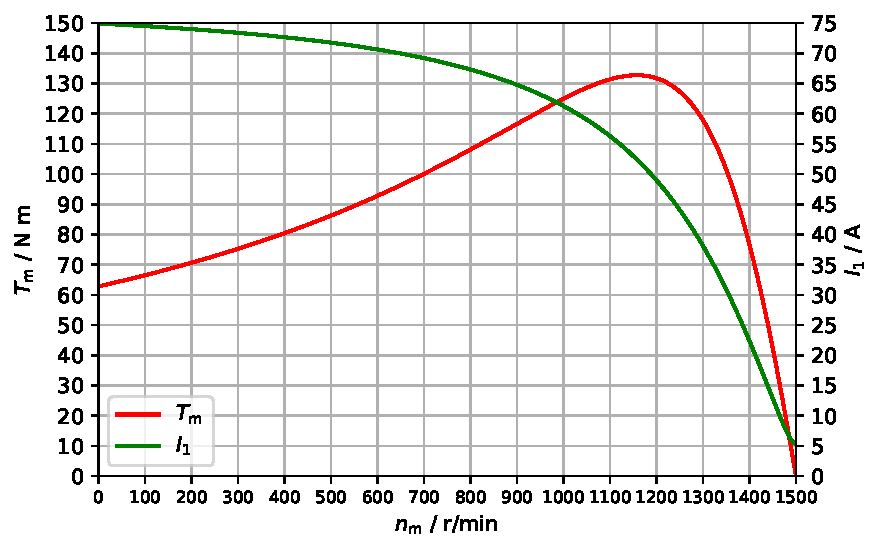
\includegraphics{Cap-PythonExemp-CaractMotor-1.pdf} $
      
    
$ 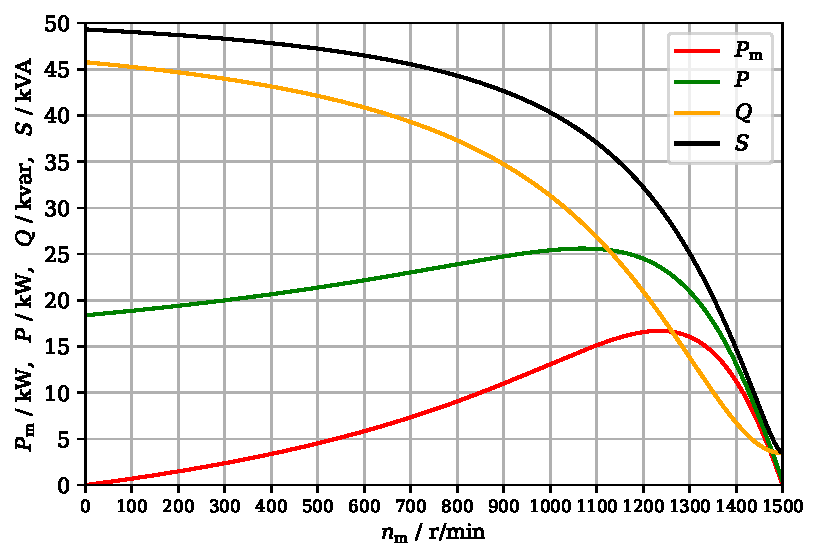
\includegraphics{Cap-PythonExemp-CaractMotor-2.pdf} $


$ 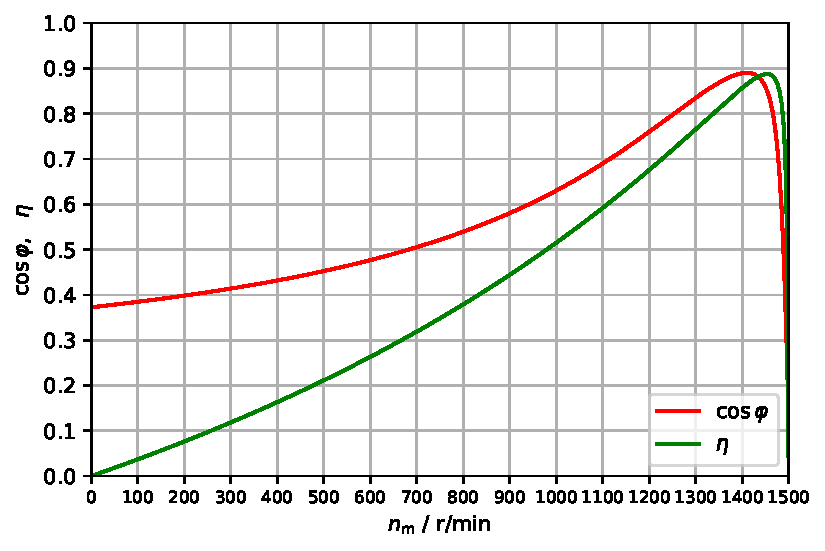
\includegraphics{Cap-PythonExemp-CaractMotor-3.pdf} $
\end{lstlisting} 






\hypertarget{exemple:TensDeseqMotor}{\subsection{Exemple \ref*{ex:TensDeseqMotor} \TensDeseqMotor}}
En el llistat \vref{lst:TensDeseqMotor} es pot veure el programa utilitzat per resoldre l'exemple \vref{ex:TensDeseqMotor}. La resolució es fa fent servir funcions del mòdul \texttt{qed.eng\_elec}. Es fa servir també la classe \texttt{Complex} del mòdul \texttt{qed.utils}.
\lstset{
	language=Python,
	numbers=left,
	frame=lines,
	morekeywords=[1]{as,None,match,case,with}
}
\lstinputlisting[caption={Python --- Exemple \ref*{ex:TensDeseqMotor} \TensDeseqMotor},label=lst:TensDeseqMotor]{Python/exemples_resolts/Exemple-10-5.py}

Quan s'executa aquest programa, el resultat que s'obté és:
\lstset{
	language=,
	numbers=none,
	frame=none
}
\begin{lstlisting}
U_AB = 399.00∠0.00° V
U_BC = 370.00∠-122.63° V
U_CA = 370.00∠122.63° V

U_AB,1 = 379.41∠0.00° V
U_AB,2 = 19.59∠0.00° V
U_AB,0 = 0.00∠0.00° V

U_AN,1 = 219.05∠-30.00° V
U_AN,2 = 11.31∠30.00° V
U_AN,2/U_AN,1 = 0.052

Z_mot,n,1 = 11.004+5.718j Ω
Z_mot,n,2 = 0.805+2.712j Ω
Z_mot,arr,1 = 1.091+2.717j Ω

I_1,n,1 = 17.66∠-57.46° A
I_1,n,2 = 4.00∠-43.47° A
I_1,n,2/I_1,n,1 = 0.226

I_1,n,A = 21.57∠-54.89° A
I_1,n,B = 17.00∠169.48° A
I_1,n,C = 15.16∠73.48° A
\end{lstlisting} 


\hypertarget{exemple:MotCarregaReduida}{\subsection{Exemple \ref*{ex:MotCarregaReduida} \MotCarregaReduida}}
En el llistat \vref{lst:MotCarregaReduida} es pot veure el programa utilitzat per resoldre l'exemple \vref{ex:MotCarregaReduida}. La resolució es fa emprant funcions del mòdul numèric \texttt{numpy} i del mòdul gràfic \texttt{matplotlib}, la funció \texttt{root\_scalar} del mòdul matemàtic \texttt{scipy.optimize}, i la classe \texttt{Motor3ph}  i la constant  \texttt{SQRT3} del mòdul \texttt{qed.eng\_elec}. La funció \texttt{root\_scalar} calcula el valor de $s$ per a diverses potències, resolent una equació no lineal; com a valor inicial per resoldre-la  s'utilitza un valor proporcional a $s\ped{n}$.
\lstset{
	language=Python,
	numbers=left,
	frame=lines,
	morekeywords=[1]{as,None,match,case,with}
}
\lstinputlisting[caption={Python --- Exemple \ref*{ex:MotCarregaReduida} \MotCarregaReduida},label=lst:MotCarregaReduida]{Python/exemples_resolts/Exemple-10-6.py}

Quan s'executa aquest programa, el resultat que s'obté és:
\lstset{
	language=,
	numbers=none,
	frame=none
}
\begin{lstlisting}[mathescape=true]
	
U_1 = 219.393 V

P_m,50% = 4526.4 W
s,50% = 0.0226

Z_mot,50% = 18.015+13.510j Ω

I_1,50% = 9.7 A
I_1,50%/I_1,n = 0.6

cos 𝜑,50% = 0.8000
η,50% = 0.8823









$ 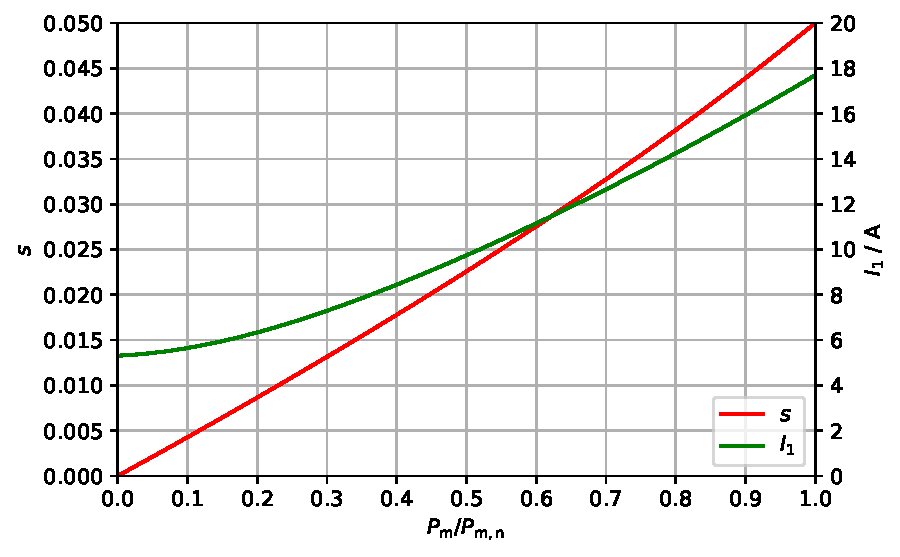
\includegraphics{Cap-PythonExemp-MotCarregaReduida-1.pdf} $




$ 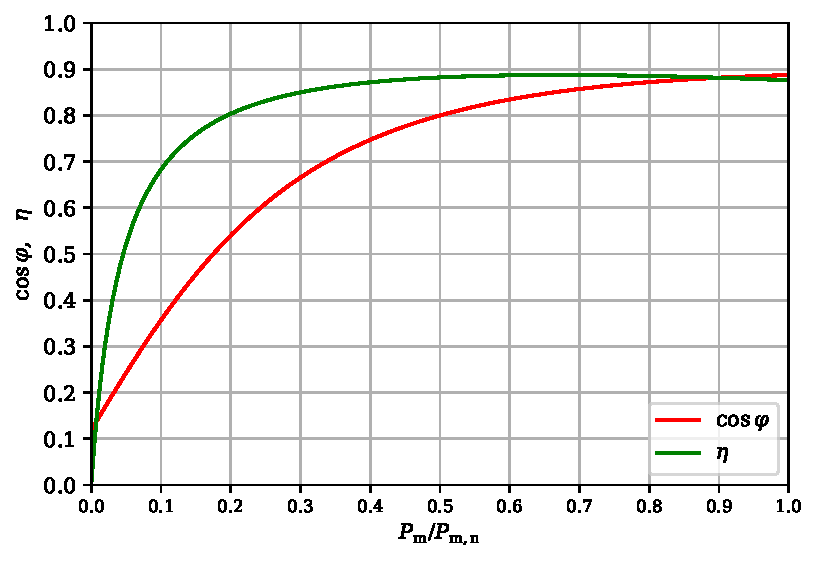
\includegraphics{Cap-PythonExemp-MotCarregaReduida-2.pdf} $
\end{lstlisting} 


\hypertarget{exemple:MotTensRedSolAp}{\subsection{Exemple \ref*{ex:MotTensRedSolAp} \MotTensRedSolAp}}
En el llistat \vref{lst:MotTensRedSolAp} es pot veure el programa utilitzat per resoldre l'exemple \vref{ex:MotTensRedSolAp}. La resolució es fa emprant funcions del mòdul numèric \texttt{numpy} i del mòdul gràfic \texttt{matplotlib}, la funció \texttt{root\_scalar} del mòdul matemàtic \texttt{scipy.optimize}, i la classe \texttt{Motor3ph}  i la constant  \texttt{SQRT3} del mòdul \texttt{qed.eng\_elec}. La funció \texttt{root\_scalar} calcula el valor de $s$ per a diverses potències, resolent una equació no lineal; com a valor inicial per resoldre-la  s'utilitza el valor $s\ped{n}$.
\lstset{
	language=Python,
	numbers=left,
	frame=lines,
	morekeywords=[1]{as,None,match,case,with}
}
\lstinputlisting[caption={Python --- Exemple \ref*{ex:MotTensRedSolAp} \MotTensRedSolAp},label=lst:MotTensRedSolAp]{Python/exemples_resolts/Exemple-10-7.py}

Quan s'executa aquest programa, el resultat que s'obté és:
\lstset{
	language=,
	numbers=none,
	frame=none
}
\begin{lstlisting}[mathescape=true]
	
P_m,n = 9052.8 W
U_1,80% = 175.514 V
s,80% = 0.0971

Z_mot,80% = 6.324+3.565j Ω

I_1,80% = 24.2 A
I_1,80%/I_1,n = 1.4

cos 𝜑,80% = 0.8711
η,80% = 0.8163
	
	
	
	
	
	
	
	
	
	
	
	
	
	
	
	
$ 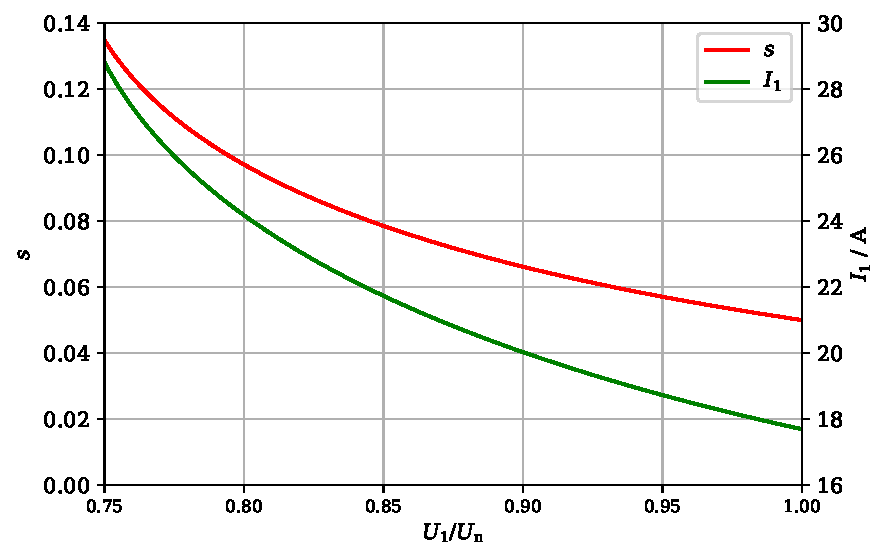
\includegraphics{Cap-PythonExemp-MotTensRedSolAp-1.pdf} $




$ 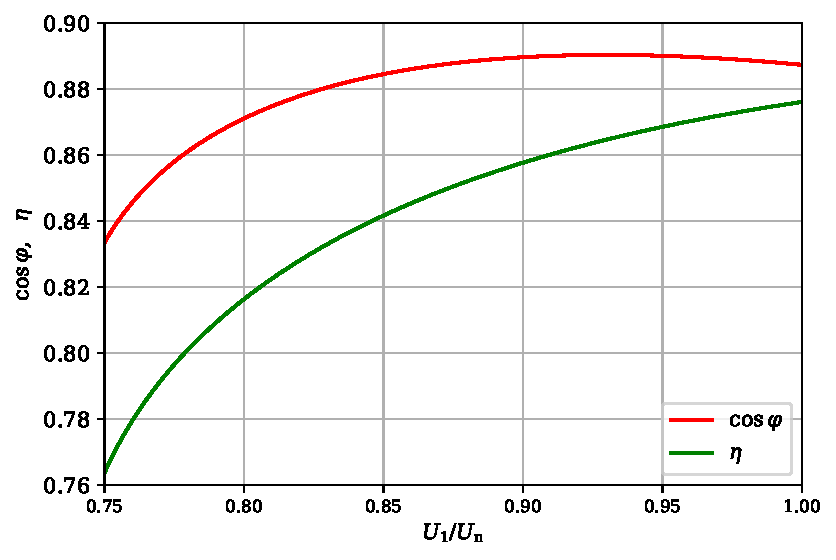
\includegraphics{Cap-PythonExemp-MotTensRedSolAp-2.pdf} $
\end{lstlisting} 



\hypertarget{exemple:MotTensRedSolEx}{\subsection{Exemple \ref*{ex:MotTensRedSolEx} \MotTensRedSolEx}}
En el llistat \vref{lst:MotTensRedSolEx} es pot veure el programa utilitzat per resoldre l'exemple \vref{ex:MotTensRedSolEx}. La resolució es fa usant funcions del mòdul numèric \texttt{numpy} i del mòdul gràfic \texttt{matplotlib},  i la classe \texttt{Motor3ph} i les constants \texttt{MOTOR} i \texttt{SQRT3} del mòdul \texttt{qed.eng\_elec}.
\lstset{
	language=Python,
	numbers=left,
	frame=lines,
	morekeywords=[1]{as,None,match,case,with}
}
\lstinputlisting[caption={Python --- Exemple \ref*{ex:MotTensRedSolEx} \MotTensRedSolEx},label=lst:MotTensRedSolEx]{Python/exemples_resolts/Exemple-10-8.py}

El programa calcula, addicionalment a l'exemple resolt a mà, els valors de la impedància del motor i  del temps que triga el motor a arrencar, al 100 \% i al 80 \% de la tensió nominal. També  representa l'evolució temporal del  corrent d'arrencada, i del parell mecànic del motor i de la càrrega, a aquestes dues tensions.

Quan s'executa aquest programa, el resultat que s'obté és:
\lstset{
	language=,
	numbers=none,
	frame=none
}
\begin{lstlisting}[mathescape=true]
	
U_1,100% = 219.393 V
U_1,80% = 175.514 V

n_m,sinc = 1500 r/min,  ω_m,sinc = 157.080 rad/s

s,100% = 0.0461
n_m,100% = 1430.8 r/min
Z_mot,100% = 11.703+6.182j Ω
I_1,100% = 16.6 A
I_1,arr,100% = 74.9 A
Tm,100% = 56.6 N·m
Tm,arr,100% = 62.8 N·m
cos 𝜑,100% = 0.8842
η,100% = 0.8797
t_arr,100% = 6.1 s

s,80% = 0.0746
n_m,80% = 1388.0 r/min
Z_mot,80% = 7.926+4.135j Ω
I_1,80% = 19.6 A
I_1,arr,80% = 59.9 A
Tm,80% = 53.4 N·m
Tm,arr,80% = 40.2 N·m
cos 𝜑,80% = 0.8866
η,80% = 0.8468
t_arr,80% = 10.4 s






$ 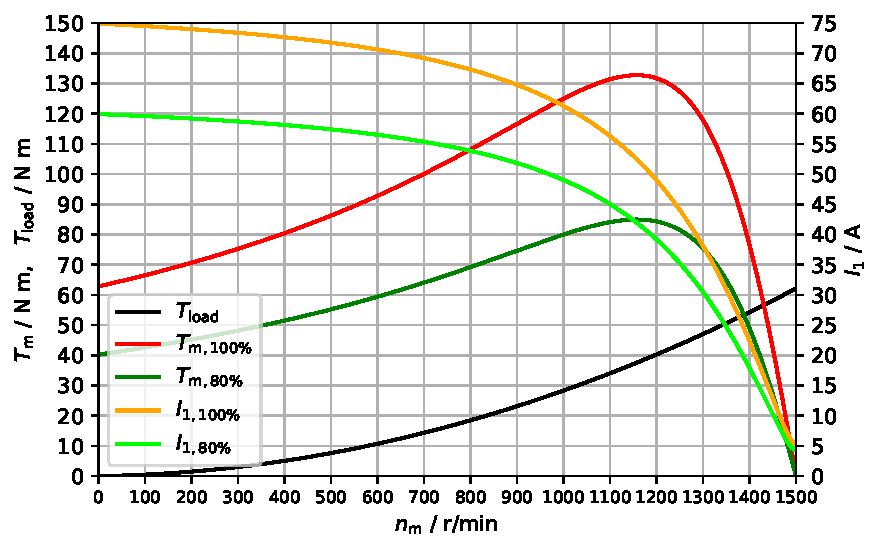
\includegraphics{Cap-PythonExemp-MotTensRedSolEx-1-1.pdf} $






$ 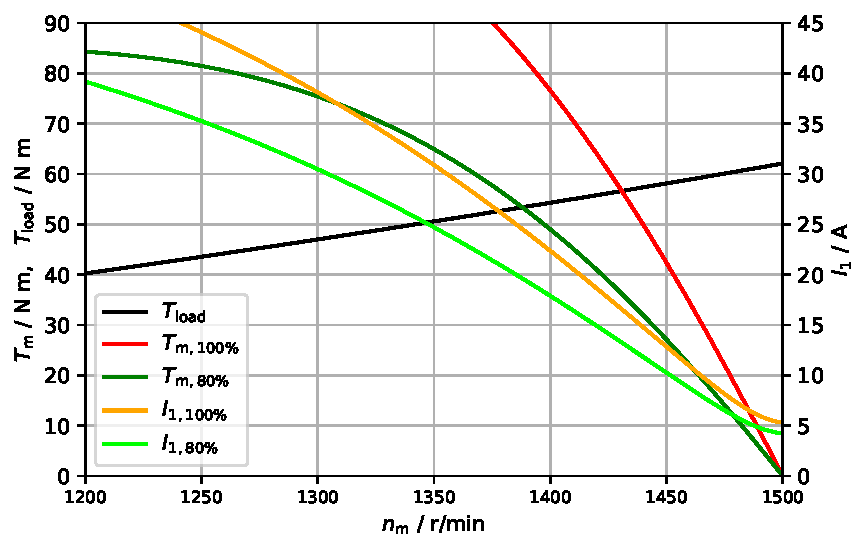
\includegraphics{Cap-PythonExemp-MotTensRedSolEx-1-2.pdf} $




$ 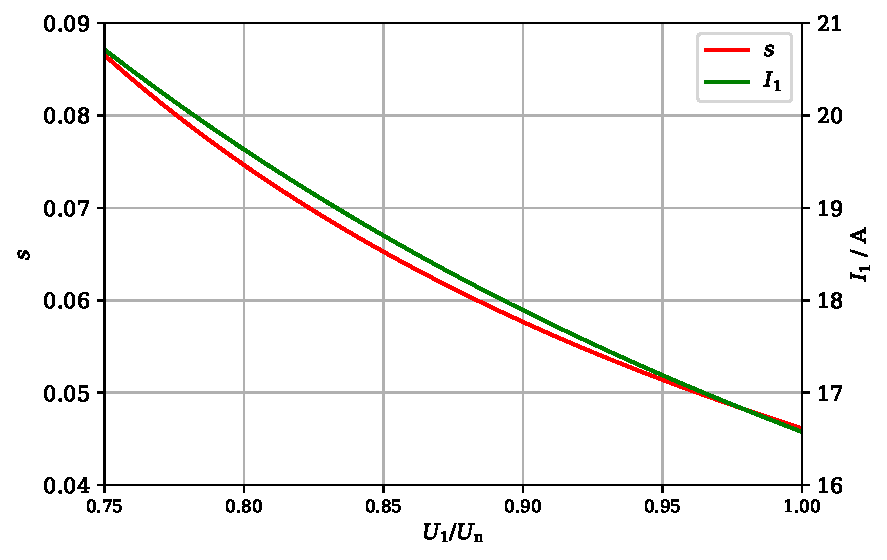
\includegraphics{Cap-PythonExemp-MotTensRedSolEx-2-1.pdf} $





$ 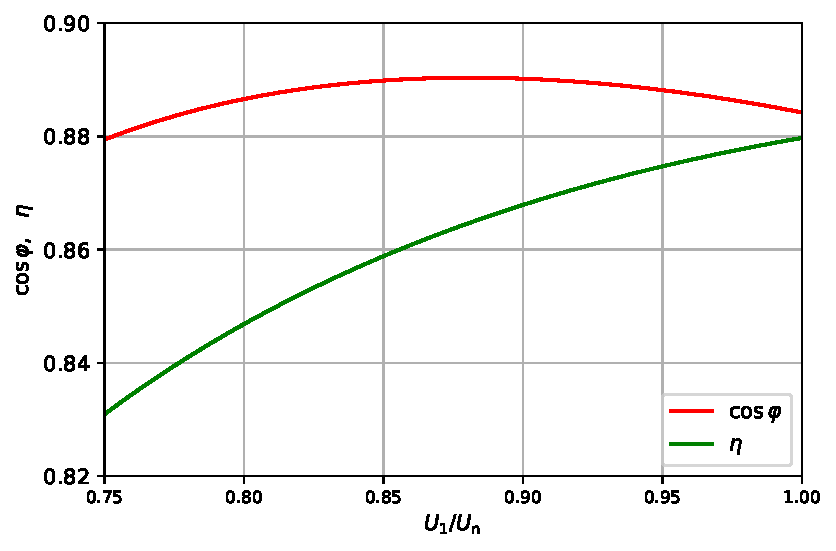
\includegraphics{Cap-PythonExemp-MotTensRedSolEx-2-2.pdf} $




$ 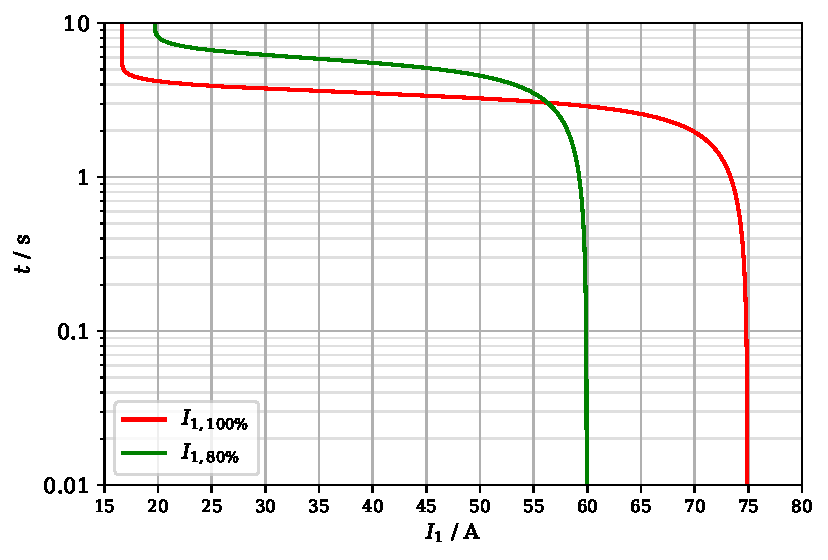
\includegraphics{Cap-PythonExemp-MotTensRedSolEx-3.pdf} $




$ 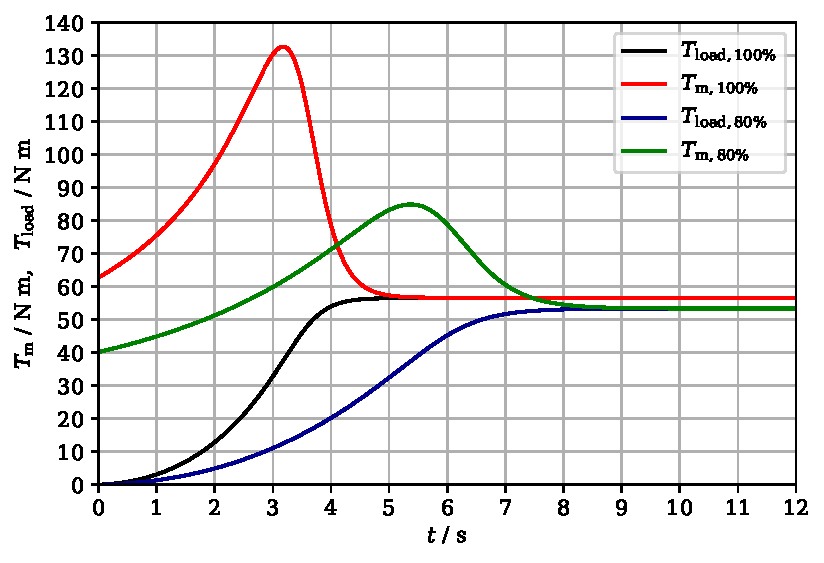
\includegraphics{Cap-PythonExemp-MotTensRedSolEx-4.pdf} $
\end{lstlisting} 



\hypertarget{exemple:MotTensRedIarr}{\subsection{Exemple \ref*{ex:MotTensRedIarr} \MotTensRedIarr}}
En el llistat \vref{lst:MotTensRedIarr} es pot veure el programa utilitzat per resoldre l'exemple \vref{ex:MotTensRedIarr}. La resolució es fa emprant funcions del mòdul numèric \texttt{numpy} i del mòdul gràfic \texttt{matplotlib}, i la classe \texttt{Motor3ph} i les constants \texttt{MOTOR} i \texttt{SQRT3}  del mòdul \texttt{qed.eng\_elec}.  Es fa servir també la classe \texttt{Complex} del mòdul \texttt{qed.utils}.
\lstset{
	language=Python,
	numbers=left,
	frame=lines,
	morekeywords=[1]{as,None,match,case,with}
}
\lstinputlisting[caption={Python --- Exemple \ref*{ex:MotTensRedIarr} \MotTensRedIarr},label=lst:MotTensRedIarr]{Python/exemples_resolts/Exemple-10-9.py}

El programa calcula, addicionalment a l'exemple resolt a mà, el valor  del temps que triga el motor a arrencar. També  representa l'evolució temporal del  corrent d'arrencada, de la tensió en el motor, i del parell mecànic del motor i de la càrrega.
Quan s'executa aquest programa, el resultat que s'obté és:
\lstset{
	language=,
	numbers=none,
	frame=none
}
\begin{lstlisting}[mathescape=true]
U_1,sist = 219.393 V
Z_sist = 0.003+0.029j Ω
Z_cable = 0.317+0.010j Ω

n_m,sinc = 1500 r/min,  ω_m,sinc = 157.080 rad/s

s,fun = 0.0485,   n_m_fun = 1427.3 r/min
U_1,fun = 214.305∠0.502° V
I_1,fun = 16.9 A
T_m,fun = 56.4 N·m

U_1,arr = 207.494∠5.238° V
I_1,arr = 70.9 A
T_m,arr = 56.2 N·m

s_T_m,max = 0.2197
n_T_m,max = 1170.5 r/min
T_m,max = 117.5 N·m

t_arr = 6.9 s
$ 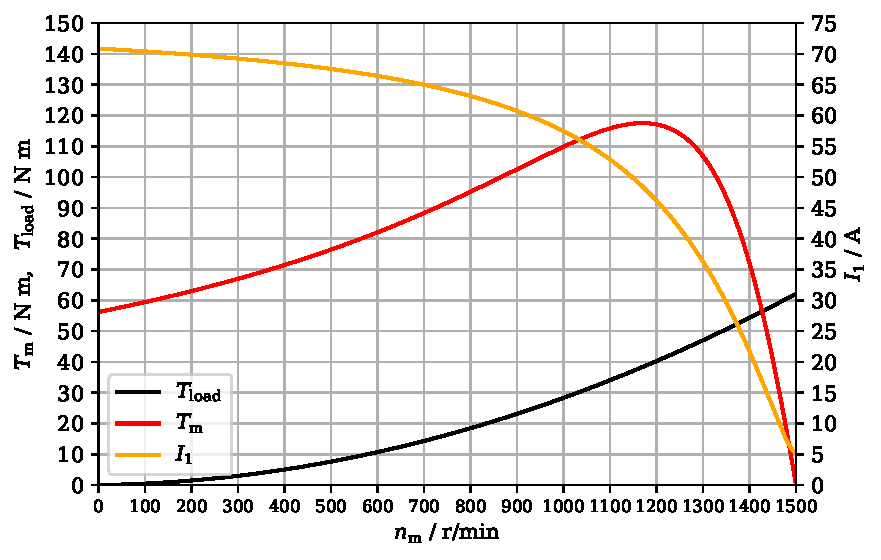
\includegraphics{Cap-PythonExemp-MotTensRedIarr-1.pdf} $

$ 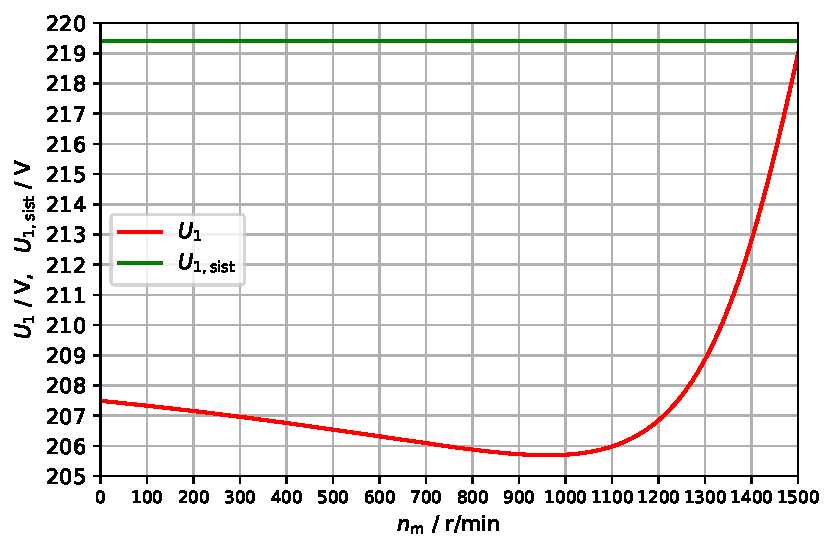
\includegraphics{Cap-PythonExemp-MotTensRedIarr-2.pdf} $





$ 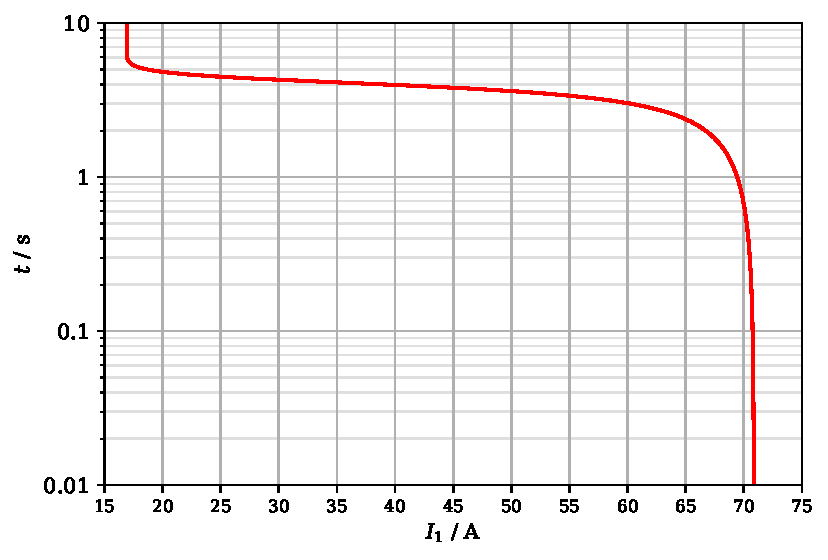
\includegraphics{Cap-PythonExemp-MotTensRedIarr-3.pdf} $



$ 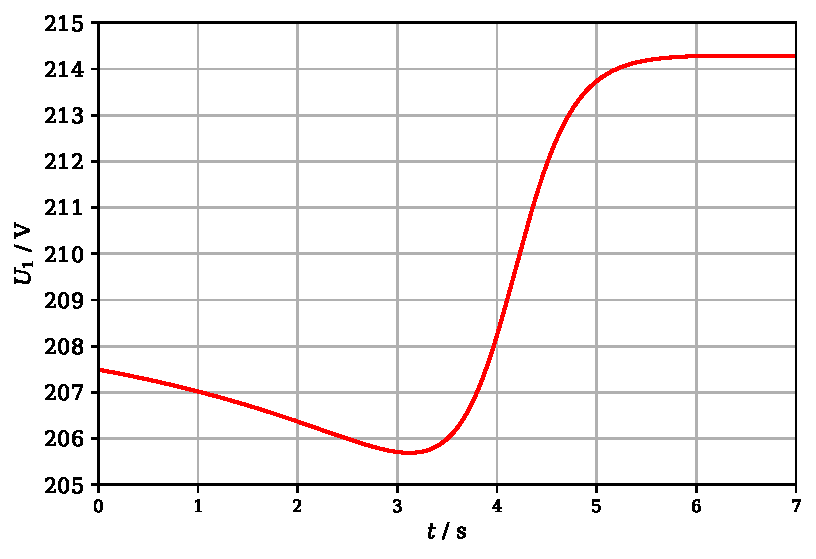
\includegraphics{Cap-PythonExemp-MotTensRedIarr-4.pdf} $

$ 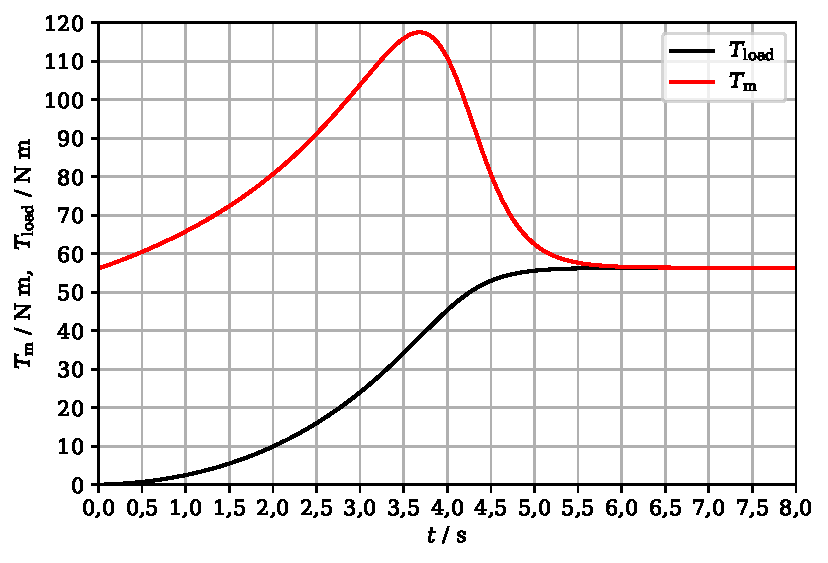
\includegraphics{Cap-PythonExemp-MotTensRedIarr-5.pdf} $
\end{lstlisting} 


\hypertarget{exemple:MotorFaseOberta}{\subsection{Exemple \ref*{ex:MotorFaseOberta} \MotorFaseOberta}}
En el llistat \vref{lst:MotorFaseOberta} es pot veure el programa utilitzat per resoldre l'exemple \vref{ex:MotorFaseOberta}. La resolució es fa emprant  la funció \texttt{A012\_to\_ABC},  la classe \texttt{Motor3ph} i la constanta \texttt{SQRT3} del mòdul \texttt{qed.eng\_elec}.  Es fa servir també la classe \texttt{Complex} del mòdul \texttt{qed.utils}.
\lstset{
	language=Python,
	numbers=left,
	frame=lines,
	morekeywords=[1]{as,None,match,case,with}
}
\lstinputlisting[caption={Python --- Exemple \ref*{ex:MotorFaseOberta} \MotorFaseOberta},label=lst:MotorFaseOberta]{Python/exemples_resolts/Exemple-10-10.py}

Quan s'executa aquest programa, el resultat que s'obté és:
\lstset{
	language=,
	numbers=none,
	frame=none
}
\begin{lstlisting}
s_n = 0.05
U_1 = 219.393 V
ω_m,sinc = 157.080 rad/s

I_1_1 = 14.7∠-21.70°
I_1_2 = 14.7∠158.30°
I_1_0 = 0.0∠0.00°

I_1_A = 0.0∠0.00°
I_1_B = 25.5∠-111.70°
I_1_C = 25.5∠68.30°

P_m = 7551.3 W
T_m = 50.6 N·m

I_1_B/I_1_n = 1.44
P_m/P_m_n = 0.83
T_m/T_m_n = 0.83	
\end{lstlisting} 



\section{Exemples del capítol \ref*{sec:ch-xarxes-elec}}

\hypertarget{exemple:XarxaAmbAcobl}{\subsection{Exemple \ref*{ex:XarxaAmbAcobl} \XarxaAmbAcobl}}
En el llistat \vref{lst:XarxaAmbAcobl} es pot veure el programa utilitzat per resoldre l'exemple \vref{ex:XarxaAmbAcobl}. Es fan servir les classes \texttt{Network},  \texttt{VoltageSource}, \texttt{CurrentSource}, \texttt{Impedance} i \texttt{MutualCoupling} del mòdul \texttt{qed.eng\_elec},  per resoldre la xarxa.
\lstset{
	language=Python,
	numbers=left,
	frame=lines,
	morekeywords=[1]{as,None,match,case,with}
}

\break

\lstinputlisting[caption={Python --- Exemple \ref*{ex:XarxaAmbAcobl} \XarxaAmbAcobl},label=lst:XarxaAmbAcobl]{Python/exemples_resolts/Exemple-11-1.py}

Quan s'executa aquest programa, el resultat que s'obté és:
\lstset{
	language=,
	numbers=none,
	frame=none
}
\begin{lstlisting}
 Branch   Nodes    Voltage / pu      Current / pu
--------  -------  ----------------  ----------------
   1      0 ► 1    1.0494∠178.5091°  0.2312∠-61.8063°
   2      0 ► 2    1.0175∠177.4776°  0.7431∠-13.0406°
   3      0 ► 3    0.9727∠169.6442°  1.2782∠-22.6715°
   4      3 ► 4    0.1495∠67.0039°   1.4946∠-22.9961°
   5      2 ► 4    0.2925∠66.2049°   0.6955∠-23.7522°
   6      2 ► 3    0.1431∠65.3702°   0.2166∠-24.9115°
   7      1 ► 2    0.0370∠28.1937°   0.2312∠-61.8063°
   8      4 ► 0    0.9512∠-19.1752°  2.1901∠-23.2362°

s_G1 = 0.1201+0.2241j
s_G2 = 0.7433+0.2484j
s_G3 = 1.2146+0.6736j
s_Q8 = 2.0781+0.1475j
\end{lstlisting} 


\hypertarget{exemple:XarxaSenseAcobl}{\subsection{Exemple \ref*{ex:XarxaSenseAcobl} \XarxaSenseAcobl}}
En el llistat \vref{lst:XarxaSenseAcobl} es pot veure el programa utilitzat per resoldre l'exemple \vref{ex:XarxaSenseAcobl}. Es fan servir les classes \texttt{Network},   \texttt{VoltageSource}, \texttt{CurrentSource} i \texttt{Impedance} del mòdul \texttt{qed.eng\_elec} per resoldre la xarxa.
\lstset{
	language=Python,
	numbers=left,
	frame=lines,
	morekeywords=[1]{as,None,match,case,with}
}
\lstinputlisting[caption={Python --- Exemple \ref*{ex:XarxaSenseAcobl} \XarxaSenseAcobl},label=lst:XarxaSenseAcobl]{Python/exemples_resolts/Exemple-11-2.py}

Quan s'executa aquest programa, el resultat que s'obté és:
\lstset{
	language=,
	numbers=none,
	frame=none
}
\begin{lstlisting}
I2 = -0.0294-3.1176j A
I5 = 0.8235-3.2059j A
\end{lstlisting} 

\hypertarget{exemple:XarxaThevenin}{\subsection{Exemple \ref*{ex:XarxaThevenin} \XarxaThevenin}}
En el llistat \vref{lst:XarxaThevenin} es pot veure el programa utilitzat per resoldre l'exemple \vref{ex:XarxaThevenin}. Es fan servir les classes \texttt{Network},  \texttt{VoltageSource}, \texttt{CurrentSource}, \texttt{Impedance} i \texttt{MutualCoupling} del mòdul \texttt{qed.eng\_elec} per resoldre la xarxa.
\lstset{
	language=Python,
	numbers=left,
	frame=lines,
	morekeywords=[1]{as,None,match,case,with}
}
\lstinputlisting[caption={Python --- Exemple \ref*{ex:XarxaThevenin} \XarxaThevenin},label=lst:XarxaThevenin]{Python/exemples_resolts/Exemple-11-3.py}

Quan s'executa aquest programa, el resultat que s'obté és:
\lstset{
	language=,
	numbers=none,
	frame=none
}
\begin{lstlisting}
E_Th(1,2) = 119.2079+2.0792j V
Z_Th(1,2) = 4.2574+2.5743j Ω
J_No(1,2) = 20.7200-12.0400j A
Y_No(1,2) = 0.1720-0.1040j S
\end{lstlisting} 


\hypertarget{exemple:CurtcircuitXarxaSenzilla}{\subsection{Exemple \ref*{ex:CurtcircuitXarxaSenzilla} \CurtcircuitXarxaSenzilla}}
En el llistat \vref{lst:CurtcircuitXarxaSenzilla} es pot veure el programa utilitzat per resoldre l'exemple \vref{ex:CurtcircuitXarxaSenzilla}. Es fan servir les classes \texttt{Network},    \texttt{VoltageSource}, \texttt{Impedance} i \texttt{ShortCircuit} del mòdul \texttt{qed.eng\_elec},  per resoldre la xarxa.

\lstset{
	language=Python,
	numbers=left,
	frame=lines,
	morekeywords=[1]{as,None,match,case,with}
}
\lstinputlisting[caption={Python --- Exemple \ref*{ex:CurtcircuitXarxaSenzilla} \CurtcircuitXarxaSenzilla},label=lst:CurtcircuitXarxaSenzilla]{Python/exemples_resolts/Exemple-11-4.py}

Quan s'executa aquest programa, el resultat que s'obté és:
\lstset{
	language=,
	numbers=none,
	frame=none
}
\begin{lstlisting}
 Branch   Nodes    Voltage / V    Current / A
--------  -------  -------------  -------------
   1      0 ► 1       -1.667          3.333
   2      2 ► 1       -1.667         -1.667
   3      1 ► 0        1.667          1.667
   4      3 ► 0       -0.667         -0.667
   5      2 ► 3        0.667          0.667
   6      3 ► 2       -0.667          1.333
   7      2 ► 0          0            2.333
\end{lstlisting}

El corrent de curtcircuit és el corresponent a la branca número 7. La tensió d'aquesta branca és, evidentment, igual a zero.

Com es pot veure, fent servir la classe   \texttt{ShortCircuit}, es pot simular  un curtcircuit en una xarxa, i es pot obtenir directament ---sense fer servir el teorema de la superposició--- el corrent de curtcircuit i el corrent que circula per cadascuna de les branques en aquesta situació.

\hypertarget{exemple:CurtcircuitXarxaComplexa}{\subsection{Exemple \ref*{ex:CurtcircuitXarxaComplexa} \CurtcircuitXarxaComplexa}}
En el llistat \vref{lst:CurtcircuitXarxaComplexa} es pot veure el programa utilitzat per resoldre l'exemple \vref{ex:CurtcircuitXarxaComplexa}. Es fan servir les classes \texttt{Network},    \texttt{VoltageSource}, \texttt{CurrentSource},  \texttt{Impedance}, \texttt{MutualCoupling} i \texttt{ShortCircuit} del mòdul \texttt{qed.eng\_elec},  per resoldre la xarxa.

\lstset{
	language=Python,
	numbers=left,
	frame=lines,
	morekeywords=[1]{as,None,match,case,with}
}

\break

\lstinputlisting[caption={Python --- Exemple \ref*{ex:CurtcircuitXarxaComplexa} \CurtcircuitXarxaComplexa},label=lst:CurtcircuitXarxaComplexa]{Python/exemples_resolts/Exemple-11-5.py}

Quan s'executa aquest programa, el resultat que s'obté és:
\lstset{
	language=,
	numbers=none,
	frame=none
}
\begin{lstlisting}
 Branch   Nodes    Voltage / V        Current / A
--------  -------  -----------------  ----------------
   1      0 ► 1    -35.2000-63.6000j  16.4800-6.3600j
   2      1 ► 2    0.0000+0.0000j     -4.2400+5.6800j
   3      2 ► 0    35.2000+63.6000j   16.9600-12.7200j
   4      1 ► 2    0.0000+0.0000j     0.0000+0.0000j
   5      0 ► 2    -35.2000-63.6000j  0.4800-6.3600j
   6      1 ► 2    0.0000+0.0000j     20.7200-12.0400j
\end{lstlisting}

El corrent de curtcircuit és el corresponent a la branca número 6. La tensió d'aquesta branca és, evidentment, igual a zero; també és nuŀla la tensió de les branques 2 i 4, ja que estan en paraŀlel amb el curtcircuit.

Igual que en l'exemple anterior, es fa servir la classe   \texttt{ShortCircuit} per obtenir directament el corrent de curtcircuit i el corrent que circula per cadascuna de les branques.


\section{Exemples del capítol \ref*{sec:ch-flux-carregues}}

\hypertarget{exemple:FluxCarrXarxa}{\subsection{Exemple \ref*{ex:FluxCarrXarxa} \FluxCarrXarxa}}
En el llistat \vref{lst:FluxCarrXarxa} es pot veure el programa utilitzat per resoldre l'exemple \vref{ex:FluxCarrXarxa}. Es fan servir dos mètodes diferents.

El primer mètode es basa en la resolució directa del sistema d'equacions no lineals de l'exemple, fent servir funcions del mòdul numèric \texttt{numpy}, del mòdul de matemàtica numèrica \texttt{scipy} i del mòdul de matemàtica simbòlica \texttt{sympy}. Primer es defineixen de forma simbòlica les variables i el sistema d'equacions a resoldre usant les funcions \texttt{symbols}, \texttt{sin} i \texttt{cos}, i després se n'obté el jacobià usant les funcions \texttt{Matrix} i \texttt{jacobian}; a continuació es fa ús de la funció  \texttt{lambdify} per crear les versions numèriques corresponents al sistema d'equacions i al jacobià, i finalment es resol el sistema amb la funció \texttt{optimize.root}. Les funcions sinus i cosinus simbòliques són  \texttt{sympy.sin} i  \texttt{sympy.cos} respectivament, no obstant això,  per tal de fer més llegible les equacions es defineixen els àlies \texttt{SIN} i \texttt{COS} per a aquestes dues funcions trigonomètriques.

El segon mètode està basat en el mòdul \texttt{pandapower}. En aquest cas s'introdueixen les dades dels components de la xarxa (generadors, línies, consums, etc.), i el flux de càrregues s'obté directament sense necessitat de plantejar cap equació. Aquest mòdul treballa amb unes unitats fixes: tensions en  \unit{kV}, potències en  \unit{MVA}, \unit{MW} i \unit{Mvar}, impedàncies longitudinals de línies en \unit{\ohm/km}, i longituds de línies en  \unit{km}. En el nostre cas, tenim una xarxa expressada amb valors en tant per u, i no coneixem els valors reals dels components. Aquesta dificultat es pot superar usant com a potència base de la xarxa \qty{1}{MVA}, assignant a tots els nusos una tensió d'\qty{1}{kV}, i assignant una longitud d'\qty{1}{km} a totes les línies; d'aquesta manera, la impedància base valdrà: $(\qty{1}{kV})^2/\qty{1}{MVA} = \qty{1}{\ohm}$. Amb aquests valors així escollits, aconseguim que els valors numèrics expressats en tant per u, siguin idèntics als valors numèrics expressats en 
\unit{kV},  \unit{MVA}, \unit{MW}, \unit{Mvar} i $\unit{\ohm/km}\times\unit{km}$, segons el cas. Els resultats, pel que fa a les potències,  segueixen dos convenis de signes; en el cas de generadors i xarxes externes, un signe positiu indica una potència activa o reactiva injectada a l'interior de la nostra xarxa; en el cas dels nusos, un signe positiu indica una potència activa o reactiva subministrada pel nus a l'exterior; i igualment en el cas d'una càrrega, un signe positiu indica una potència activa o reactiva absorbida per la càrrega ---o sigui, subministrada  pel nus.
\lstset{
	language=Python,
	numbers=left,
	frame=lines,
	morekeywords=[1]{as,None,match,case,with}
}
\lstinputlisting[caption={Python --- Exemple \ref*{ex:FluxCarrXarxa} \FluxCarrXarxa},label=lst:FluxCarrXarxa]{Python/exemples_resolts/Exemple-12-1.py}

Quan s'executa aquest programa, el resultat que s'obté és:
\lstset{
	language=,
	numbers=none,
	frame=none
}
\begin{lstlisting}
δ_2 = -0.015277 rad = -0.875336°
v_3 = 1.033587
δ_3 = -0.014301 rad = -0.819384°

s_1 = 0.85681+0.52171j
s_2 = -0.25000-0.20049j
s_G1 = 0.85681+0.52171j
s_G2 = 0.25000+0.04951j

Tensions i potències del nusos
      vm_pu  va_degree     p_mw    q_mvar
1  1.050000   0.000000 -0.85681 -0.521705
2  1.030000  -0.875336  0.25000  0.200493
3  1.033587  -0.819384  0.60000  0.300000

Potència injectada al nus 1 per la xarxa externa
      p_mw    q_mvar
1  0.85681  0.521705

Potència injectada al nus 2 pel generador
   p_mw    q_mvar  va_degree  vm_pu
2  0.25  0.049507  -0.875336   1.03
\end{lstlisting} 


\hypertarget{exemple:ControlTensCond}{\subsection{Exemple \ref*{ex:ControlTensCond} \ControlTensCond}}
En el llistat \vref{lst:ControlTensCond} es pot veure el programa utilitzat per resoldre l'exemple \vref{ex:ControlTensCond}. Es fan servir dos mètodes diferents.

El primer mètode es basa en la resolució directa dels sistemes d'equacions no lineals de l'exemple. Per resoldre l'apartat a)   es fan servir funcions del mòdul numèric \texttt{numpy}, del mòdul de matemàtica numèrica \texttt{scipy} i del mòdul de matemàtica simbòlica \texttt{sympy}. Primer es defineixen de forma simbòlica les variables i el sistema d'equacions a resoldre usant les funcions \texttt{symbols}, \texttt{sin} i \texttt{cos}, i després se n'obté el jacobià usant les funcions \texttt{Matrix} i \texttt{jacobian}; a continuació es fa ús de la funció  \texttt{lambdify} per crear les versions numèriques corresponents al sistema d'equacions i al jacobià, i finalment es resol el sistema amb la funció \texttt{optimize.root}. L'apartat b) de l'exemple es resol de forma similar, però com que només tenim una equació, en lloc de les funcions \texttt{Matrix}, \texttt{jacobian} i \texttt{optimize.root}, es fan servir les funcions \texttt{diff} i \texttt{optimize.root\_scalar}. Les funcions sinus i cosinus simbòliques són  \texttt{sympy.sin} i  \texttt{sympy.cos} respectivament, no obstant això,  per tal de fer més llegible les equacions es defineixen els àlies \texttt{SIN} i \texttt{COS} per a aquestes dues funcions trigonomètriques.

El segon mètode està basat en el mòdul \texttt{pandapower}. Són d'aplicació les mateixes consideracions de l'exemple anterior, sobre les unitats que cal utilitzar. En aquest cas tenim addicionalment l'admitància transversal d'una línia, que \texttt{pandapower} requereix que s'expressi en \unit{nF/km}; ens caldrà doncs dividir el nostre valor d'admitància en tant per u, per $2 \pi f$ (amb $f = \qty{50}{Hz}$), i multiplicar el resultat per $10^9$, per tal d'obtenir el valor en les unitats necessàries. En el cas de l'apartat  b) de l'exemple, el banc de condensadors es modela com un generador connectat al nus 2, amb una potència activa  igual a zero.
\lstset{
	language=Python,
	numbers=left,
	frame=lines,
	morekeywords=[1]{as,None,match,case,with}
}


\lstinputlisting[caption={Python --- Exemple \ref*{ex:ControlTensCond} \ControlTensCond},label=lst:ControlTensCond]{Python/exemples_resolts/Exemple-12-2.py}

Quan s'executa aquest programa, el resultat que s'obté és:
\lstset{
	language=,
	numbers=none,
	frame=none
}
\begin{lstlisting}
Cas a)
---------------------------------------------
v_2 = 0.970306
δ_2 = -0.060222 rad = -3.450451°

s_12 = 0.82813+0.59423j
s_G1 = 2.02813+0.89423j

Tensions i potències del nusos
      vm_pu  va_degree      p_mw    q_mvar
1  1.050000   0.000000 -0.828126 -0.594232
2  0.970306  -3.450451  0.800000  0.600000

Potència injectada al nus 1 per la xarxa externa
       p_mw    q_mvar
1  2.028126  0.894232


Cas b)
---------------------------------------------
δ_2 = -0.072323 rad = -4.143827°

s_12 = 0.81695-0.04520j
s_21 = -0.80000-0.00484j
s_G1 = 2.01695+0.25480j
s_C2 = -0.00000+0.59516j

Tensions i potències del nusos
   vm_pu  va_degree      p_mw    q_mvar
1   1.05   0.000000 -0.816953  0.045202
2   1.03  -4.143827  0.800000  0.004844

Potència injectada al nus 1 per la xarxa externa
       p_mw    q_mvar
1  2.016953  0.254798

Potència injectada al nus 2 pel banc de condensadors
   p_mw    q_mvar  va_degree  vm_pu
2   0.0  0.595156  -4.143827   1.03
\end{lstlisting} 


\hypertarget{exemple:ControlTensTrafo}{\subsection{Exemple \ref*{ex:ControlTensTrafo} \ControlTensTrafo}}
En el llistat \vref{lst:ControlTensTrafo} es pot veure el programa utilitzat per resoldre l'exemple \vref{ex:ControlTensTrafo}. Es fan servir dos mètodes diferents.

El primer mètode es basa en la resolució directa del sistema d'equacions no lineals de l'exemple, fent servir funcions  del mòdul de matemàtica numèrica \texttt{scipy} i del mòdul de matemàtica simbòlica \texttt{sympy}. Primer es defineixen de forma simbòlica les variables i el sistema d'equacions a resoldre usant les funcions \texttt{symbols}, \texttt{sin} i \texttt{cos}, i després se n'obté el jacobià usant les funcions \texttt{Matrix} i \texttt{jacobian}; a continuació es fa ús de la funció  \texttt{lambdify} per crear les versions numèriques corresponents al sistema d'equacions i al jacobià, i finalment es resol el sistema amb la funció \texttt{optimize.root}.

El segon mètode està basat en el mòdul \texttt{pandapower}. Són d'aplicació les mateixes consideracions dels exemples anteriors, sobre les unitats que cal utilitzar. En aquest cas tenim addicionalment un transformador, al qual li assignarem una potència d'\qty{1}{MVA}, i una tensió primària i secundària d'\qty{1}{kV}; amb aquests valors, només caldrà multiplicar per 100 la impedància en tant per u  del transformador per tal d'obtenir el valor en tant per cent, que requereix \texttt{pandapower}. A més, atès que el que busquem és la relació de transformació del transformador, és obligat definir quan es crea el transformador, els paràmetres: \texttt{tap\_side='hv'}, \texttt{tap\_step\_percent=1}, \texttt{tap\_min=--10}, \texttt{tap\_max=10}, \texttt{tap\_neutral=0} i  \texttt{tap\_pos=0}; els valors de \texttt{tap\_min} i \texttt{tap\_max} són arbitraris, però han de ser prou grans perquè el valor final calculat de \texttt{tap\_pos} quedi dins del marge que defineixen. Addicionalment, cal fer servir la funció \texttt{ContinuousTapControl} del mòdul \texttt{pandapower.control}, inicialitzant-la amb el valor \texttt{vm\_set\_pu=1}, que és el valor del mòdul de la tensió que volem mantenir en el secundari del transformador.
\lstset{
	language=Python,
	numbers=left,
	frame=lines,
	morekeywords=[1]{as,None,match,case,with}
}

\break

\lstinputlisting[caption={Python --- Exemple \ref*{ex:ControlTensTrafo} \ControlTensTrafo},label=lst:ControlTensTrafo]{Python/exemples_resolts/Exemple-12-3.py}

Quan s'executa aquest programa, el resultat que s'obté és:
\lstset{
	language=,
	numbers=none,
	frame=none
}
\begin{lstlisting}
δ_2 = -0.039196 rad = -2.245743°
m = 0.979639

Tensions i potències del nusos
   vm_pu  va_degree  p_mw  q_mvar
1    1.0   0.000000  -2.0    -1.1
2    1.0  -2.245744   2.0     1.0

Posició del "tap" = -2.036057
Relació de transformació = 0.979639
\end{lstlisting}

El valor calculat de \texttt{tap\_pos} està dins dels marges establerts (entre $-10$ i 10, en el nostre cas); si no fos així, la tensió del nus 2 no hauria arribat al valor fixat de \qty{1}{pu}, i caldria augmentar aquests marges.




\section{Exemples del capítol \ref*{sec:ch-normes}}

\hypertarget{exemple:ProtInvIntVar}{\subsection{Exemple \ref*{ex:ProtInvIntVar} \ProtInvIntVar}}
En el llistat \vref{lst:ProtInvIntVar} es pot veure el programa utilitzat per resoldre l'exemple \vref{ex:ProtInvIntVar}. Es fan servir funcions  del mòdul numèric \texttt{numpy}, del mòdul de matemàtica numèrica \texttt{scipy} i del mòdul gràfic \texttt{matplotlib}. A partir de l'equació \eqref{eq:50-51}, es fa servir la funció  \texttt{optimize.root} del mòdul \texttt{scipy} per trobar el valor de $\tauup$ que compleix: $\int_0^\tauup \frac{1}{t_{51}(I(t))}  \diff t - 1 = 0$; aquesta  funció requereix un valor inicial de la solució, a partir del qual comença a calcular-ne el valor exacte. Si mirem la gràfica de l'exemple \ref{ex:ProtInvIntVar}, veiem a ull que el corrent inicial és d'uns \qty{30}{kA}, i que amb aquest valor mantingut la funció 51 actuaria en uns \qty{0,22}{s}; atès que el temps d'actuació ha de ser superior a aquest valor, farem servir \qty{0,25}{s} com a valor inicial per a la funció \texttt{optimize.root}. Aquesta funció, a més de la solució numèrica, també  dona informació addicional; en particular, el paràmetre booleà \texttt{success} indica si s'ha obtingut o no una solució correcta, i el  paràmetre de text \texttt{message}  dona informació sobre la solució obtinguda. La integral $\int_0^\tauup \frac{1}{t_{51}(I(t))}  \diff t$ es calcula amb la funció \texttt{integrate.quad} del mòdul \texttt{scipy}, que dona resultats més precisos que la integració pel mètode dels trapezis.
\lstset{
	language=Python,
	numbers=left,
	frame=lines,
	morekeywords=[1]{as,None,match,case,with}
}
\lstinputlisting[caption={Python --- Exemple \ref*{ex:ProtInvIntVar} \ProtInvIntVar},label=lst:ProtInvIntVar]{Python/exemples_resolts/Exemple-13-1.py}

Quan s'executa aquest programa, el resultat que s'obté és:
\lstset{
	language=,
	numbers=none,
	frame=none
}
\begin{lstlisting}[mathescape=true]
$ 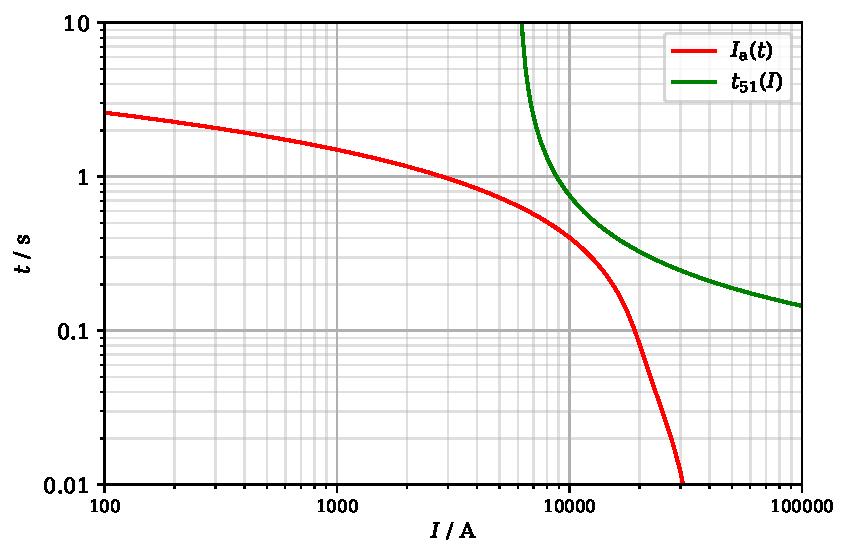
\includegraphics{Cap-PythonExemp-ProtInvIntVar.pdf} $

T = 0.6
-----------------------------------
Temps calculat d'actuació: 0.4096 s
Valor de la integral: 1.0000

message: The solution converged.
success: True
 status: 1
    fun: -2.220446049250313e-16
      x: [ 4.096e-01]
 method: hybr
   nfev: 9
   fjac: [[-1.000e+00]]
      r: [-1.288e+00]
    qtf: [ 1.297e-13]

T = 0.8
-----------------------------------
Temps calculat d'actuació: 0.6462 s
Valor de la integral: 0.8647

message: The iteration is not making good progress, as measured by the 
         improvement from the last ten iterations.
success: False
 status: 5
    fun: -0.13533445834807267
      x: [ 6.462e-01]
 method: hybr
   nfev: 26
   fjac: [[-1.000e+00]]
      r: [-1.634e-04]
    qtf: [ 1.353e-01]
\end{lstlisting}


En aquest programa es resolen dos casos. El primer ---amb  T = 0,6 en la funció $t_{51}(I)$--- és el mateix que el de l'exemple resolt a mà; el valor \texttt{True} del paràmetre \texttt{success} i el text  \texttt{«The solution converged.»} del paràmetre \texttt{message}, confirmen que el valor calculat de \qty{0,4096}{s} és correcte, i que, per tant, la protecció 51 actua; una altra constatació del fet que la protecció actua, és el valor de la integral igual a 1. En el Segon cas ---amb T = 0,8 en la funció $t_{51}(I)$--- el valor \texttt{False} del paràmetre \texttt{success}, i el text  \texttt{«The iteration is not making good progress, as measured by the improvement from the last ten iterations.»} del paràmetre \texttt{message}, indiquen que el valor calculat de \qty{0,6462}{s} no és correcte, i que, per tant, la protecció 51 no actua; una altra ratificació del fet que la protecció no actua, és el valor de la integral de 0,8647, menor que 1. 


\section{Exemples de l'apèndix \ref*{sec:ch-calc-num}}

\hypertarget{exemple:InterpLinCub}{\subsection{Exemple \ref*{ex:InterpLinCub} \InterpLinCub}}
En el llistat \vref{lst:InterpLinCub} es pot veure el programa utilitzat per resoldre l'exemple \vref{ex:InterpLinCub}. Es fa servir la funció \texttt{interp1d} del mòdul \texttt{scipy.interpolate} per fer la interpolació. També s'utilitzen funcions dels mòduls \texttt{numpy} i  \texttt{matplotlib}.
\lstset{
	language=Python,
	numbers=left,
	frame=lines,
	morekeywords=[1]{as,None,match,case,with}
}


\lstinputlisting[caption={Python --- Exemple \ref*{ex:InterpLinCub} \InterpLinCub},label=lst:InterpLinCub]{Python/exemples_resolts/Exemple-D-1.py}

El programa mostra, addicionalment a l'exemple resolt a mà, una gràfica amb la funció $y=\sin(x)$, els punts d'interpolació i les corbes d'interpolació lineal i cúbica. 
Quan s'executa aquest programa, el resultat que s'obté és:
\lstset{
	language=,
	numbers=none,
	frame=none
}
\begin{lstlisting}[mathescape=true]
Interpolació lineal: 0.9975. Interpolació cúbica: 1.0000

$ 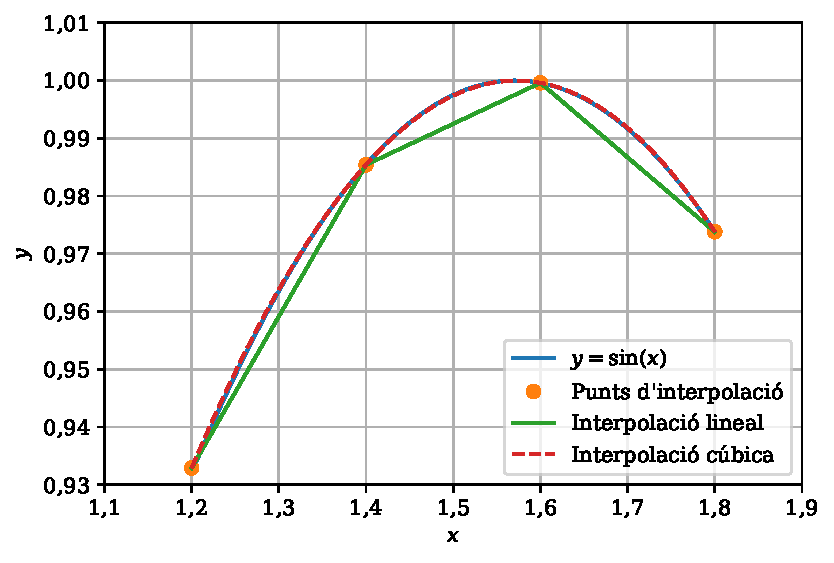
\includegraphics{Cap-PythonExemp-Interpol.pdf} $
\end{lstlisting} 


\hypertarget{exemple:InterpDuesDim}{\subsection{Exemple \ref*{ex:InterpDuesDim} \InterpDuesDim}}
En el llistat \vref{lst:InterpDuesDim} es pot veure el programa utilitzat per resoldre l'exemple \vref{ex:InterpDuesDim}. A més de la interpolació lineal, també es fa servir la interpolació cúbica ---més precisa--- per resoldre l'exemple. S'utilitza la funció \texttt{RegularGridInterpolator} del mòdul \texttt{scipy.interpolate} per fer la interpolació. També s'utilitzen funcions dels mòduls \texttt{numpy} i  \texttt{matplotlib}.
\lstset{
	language=Python,
	numbers=left,
	frame=lines,
	morekeywords=[1]{as,None,match,case,with}
}
\lstinputlisting[caption={Python --- Exemple \ref*{ex:InterpDuesDim} \InterpDuesDim},label=lst:InterpDuesDim]{Python/exemples_resolts/Exemple-D-2.py}

El programa mostra, addicionalment a l'exemple resolt a mà, una gràfica amb els punts d'interpolació i la superfície d'interpolació cúbica.

Quan s'executa aquest programa, el resultat que s'obté és:
\lstset{
	language=,
	numbers=none,
	frame=none
}
\begin{lstlisting}[mathescape=true]
Interpolació lineal: 4.20 cP

Interpolació cúbica: 4.12 cP

$ 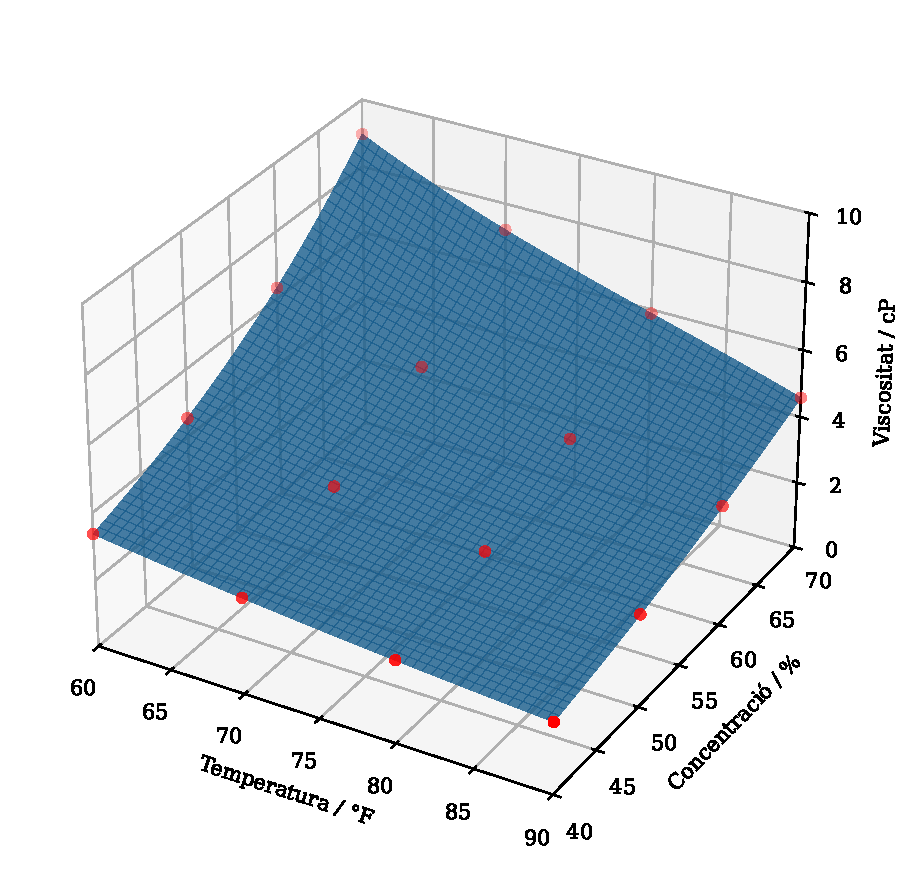
\includegraphics{Cap-PythonExemp-InterpolDuesDim.pdf} $
\end{lstlisting} 


La  funció  \texttt{RegularGridInterpolator} requereix un nombre de punts  mínim $n$, per a cada eix d'interpolació: $n \geq k+1$, amb $k=1$ per a una interpolació lineal, $k=3$ per a una interpolació cúbica, i $k=5$ per a una interpolació de cinquè grau. En el nostre cas tenim $n=4$ punts per a cada eix (variables \texttt{temp} i \texttt{conc}), que són el mínim necessari en el cas de $k=3$.

\hypertarget{exemple:IntegracioNum}{\subsection{Exemple \ref*{ex:IntegracioNum} \IntegracioNum}}
En el llistat \vref{lst:IntegracioNum} es pot veure el programa utilitzat per resoldre l'exemple \vref{ex:IntegracioNum}. A més de la integració amb els  mètodes dels trapezis i de Simpson ---amb les funcions \texttt{trapezoid} i \texttt{simpson} del mòdul \texttt{scipy.integrate}--- també es fa servir la funció  d'integració genèrica \texttt{quad} del mateix mòdul,  la qual usa l'equació de la funció que es vol integrar, i torna la integral i una estimació de l'error. Atès que la funció a integrar té una primitiva coneguda, utilitzarem també la funció \texttt{integrate} del mòdul de matemàtica simbòlica \texttt{sympy} per calcular la integral de forma exacta.
\lstset{
	language=Python,
	numbers=left,
	frame=lines,
	morekeywords=[1]{as,None,match,case,with}
}
\lstinputlisting[caption={Python --- Exemple \ref*{ex:IntegracioNum} \IntegracioNum},label=lst:IntegracioNum]{Python/exemples_resolts/Exemple-D-3.py}

Quan s'executa aquest programa, el resultat que s'obté és:
\lstset{
	language=,
	numbers=none,
	frame=none
}
\begin{lstlisting}
Integral (trapezoid) = 0.6956
Integral (simpson) = 0.6932
Integral (quad) = 0.6931471805599454, Error = 7.70e-15
Integral (simbòlica) = log(2) = 0.693147180559945309417232121458
\end{lstlisting} 

Cal tenir en compte que en la simbologia del mòdul \texttt{sympy}, \texttt{log(x)} representa un logaritme neperià; un logaritme decimal es representa com \texttt{log(x, 10)}.

La funció \texttt{simpson}  pot treballar amb divisions d'amplada diferent, i amb un nombre de punts que tant pot ser parell com senar.

L'estimació de l'error de la funció \texttt{quad} és prou bona, només cal comparar el valor obtingut de la integral  amb el valor exacte amb 30 decimals.


\hypertarget{exemple:SolFunNoLin}{\subsection{Exemple \ref*{ex:SolFunNoLin} \SolFunNoLin}}
En el llistat \vref{lst:SolFunNoLin} es pot veure el programa utilitzat per resoldre l'exemple \vref{ex:SolFunNoLin}. Primer es defineix la funció $f(x)$ i la seva funció derivada, i després es fa servir la funció \texttt{root\_scalar}  del mòdul \texttt{scipy.optimize} per trobar la solució de $f(x)=0$, amb els mètodes de Newton i de la secant. A continuació es resol el mateix problema utilitzant el mòdul  de matemàtica simbòlica \texttt{sympy} a partir de la funció \texttt{symbols}, que crea variables simbòliques, de la funció \texttt{diff}, que calcula de forma simbòlica la derivada d'una funció, i de la funció  \texttt{lambdify}, que crea funcions numèriques a partir de funcions simbòliques.
\lstset{
	language=Python,
	numbers=left,
	frame=lines,
	morekeywords=[1]{as,None,match,case,with}
}


\lstinputlisting[caption={Python --- Exemple \ref*{ex:SolFunNoLin} \SolFunNoLin},label=lst:SolFunNoLin]{Python/exemples_resolts/Exemple-D-4.py}

Quan s'executa aquest programa, el resultat que s'obté és:
\lstset{
	language=,
	numbers=none,
	frame=none
}
\begin{lstlisting}
Resolució numèrica
----------------------------------------------------------------
Newton: x = 0.01742101588983377 , f(x) = -1.0913936421275139e-11
Secant: x = 0.017421015887729187 , f(x) = 1.7249829397769645e-05

Resolució simbòlica + numèrica
----------------------------------------------------------------
Newton: x = 0.01742101588983377 , f(x) = -1.0913936421275139e-11
Secant: x = 0.017421015887729187 , f(x) = 1.7249829397769645e-05
\end{lstlisting} 
